%!TEX encoding = UTF-8 Unicode
%!TEX program = xelatex

\documentclass[bachelor]{ustcthesis}
% bachelor|master|doctor
\usepackage{ustcextra}
\graphicspath{{figures/}}
% \bibliographystyle{ustcauthoryear}
\bibliographystyle{ustcnumerical}

\title{一种关于数据立方体的相关并行算法模型及优化方案}
\author{邹凯}
\major{计算机专业}
\advisor{谢希科\ 教授}
\submitdate{二〇一七年六月}
%\secrettext{机密\quad 小于等于20年}   % 内部|秘密|机密,注释本行则不保密
\depart{中国科学技术大学\ 计算机科学与技术学院}

\entitle{A parallel approach and its optimization for data cubes}
\enauthor{Kai Zou}
\enmajor{Computer Science}
\enadvisor{Prof. Xike\ Xie}
\ensubmitdate{June, 2017}
%\ensecrettext{Confidential\quad Less than or equal to 20 years}  % Internal|Secret|Confidential

\begin{document}

\maketitle

%
% 本科论文:
%   frontmatter: 致谢、目录、中文摘要、英文摘要
%   mainmatter: 正文章节、参考文献
%   appendix: 附录
%
% 硕博论文:
%   frontmatter: 中文摘要、英文摘要、目录、符号说明
%   mainmatter: 正文、参考文献
%   appendix: 附录
%   backmatter: 致谢、发表论文
%

\frontmatter
\begin{acknowledgements}

自接触计算机领域以来,我就一直对高性能计算领域抱有浓厚的兴趣。每当看到一个思路敏捷的算法,抑或是一个精妙的实现,我都会认真将其记录下来,在之后细细品读。无论是从算法本身的设计上,还是从如何挖掘新兴的软硬件设施的潜力上,总会有一些厉害的前辈,或者是同辈,甚至可能是后辈们,在不经意间,给予我极大的灵光。

我想,所谓计算机科学的艺术,大概就是这样的吧。

本科的毕业论文,以这个方面的相关研究作为主题,也算是对本科数年,自己寻找的前进方向的一个答复吧。

在论文成文的过程中,我得到了我的导师,中国科学技术大学的谢希科教授的大力支持与帮助。无数次的方向研讨meeting,无数次的交流,这每一分每一秒都包含着老师的心血,包含着老师的智慧。

而说起为何踏进数据库这个领域,选择在数据库这个领域走高性能研究的路子,那是因为有两位至关重要的前辈,充当了我在这个领域的领路人。一位是谢希科教授,另一位则是新加坡国立大学的何炳胜副教授。这两位杰出的前辈,一同向我展示了数据库领域的博大精深,更重要的是,一同向我展现了,一个合格的学术大师应有的风貌。

同时,我也要感谢在新加坡国立大学实习时的诸位前辈们。是优秀的你们给予了我奋发向上,与你们并肩作战的动力。

我还要感谢无时无刻不在给予我无微不至的关怀的家人们,以及愿意与我分享生活中点点滴滴的喜怒哀乐的朋友们。是你们,让我的生活变得更加安逸舒适,变得更加多姿多彩。

最后,请容许我用一句话,结束这冗长无味但是真挚的致谢,同时拉开新生活的帷幕

\emph{——而那过去了的,就会成为亲切的怀恋}

\end{acknowledgements}

\tableofcontents
\begin{abstract}
本文是中国科学技术大学本硕博毕业论文 \LaTeX{} 模板示例文件。本模板由
zepinglee和seisman创建,其前身是ywg@USTC创建的本硕博论文通用模板。
本模板遵循中国科学技术大学的论文写作规范,适用于撰写学士、硕士和博士学位论文。

本示例文档中会演示如何使用 \LaTeX{} 的一些基本命令以及本模板提供的一些特殊功能,
模板的选项及详细用法请参考模板说明文档 ustcthesis.pdf。

\keywords{中国科学技术大学\zhspace{} 学位论文\zhspace{} \LaTeX{}~通用模板\zhspace{} 学士\zhspace{}
硕士\zhspace{} 博士\zhspace{} 示例文档\zhspace{} 模板说明文档}
\end{abstract}

\begin{enabstract}
This is a sample document of USTC thesis \LaTeX{} template for bachelor, master
and doctor. The template is created by zepinglee and seisman, which orignate from
the template created by ywg@USTC\@. The template meets the equirements of USTC
theiss writing standards.

This document will show the usage of basic commands provided by \LaTeX{} and some
features provided by the template. For more information, please refer to the
template document ustcthesis.pdf.

\enkeywords{University of Science and Technology of China (USTC), Thesis, Universal \LaTeX{} Template, Bachelor, Master, PhD}
\end{enabstract}

\listoffigures
\listoftables
\listofalgorithms  % 算法索引,如不需要,可直接注释掉本行
% \begin{notation}

\centering
\begin{tabular}{rl}
$\ln x$ & natural logarithm $\log_ex$ \\
$\log x$ & common logarithm $\log_{10}x$ \\
$x\ \mathrm{mod}\ y$ & remainder \\
\end{tabular}

\end{notation}


\mainmatter
\chapter{简介}
\section{模板简介}
测试脚注\footnote{分别编号}。

\subsection{模板介绍1}

\subsubsection{模板测试}

\subsection{模板介绍2}

\section{系统要求}

\section{问题反馈}
测试脚注\footnote{脚注2}

\chapter{背景工作与研究动机}
\citestyle{ustcnumerical}
\section{Parallel-Database相关}

并行计算是一个发展历史悠久的领域,其最早的发源要追寻到上世纪五十年代后期。上世纪六十年代至七十年代,共享内存的多处理器体系结构出现了。在上世纪八十年代,大规模并行处理器的出现开始占领市场,然而旋即又被集群所取代。发展至今天,并行计算硬件的主流已经成为了多核处理器\cite{ManycoreShift}

在这个主流下,越来越多的硬件被发掘出来参与到并行计算中来。图形处理器(GPU)最初是被开发来实现以电子显示为主的各方面的图形演算与生成的,然而由于其架构满足流水线深,可利用核心多等特点,很快人们就开始研究GPU的通用用途(GPGPU),其中一个很重要的领域就是GPU参与的并行计算。2006年,NVIDIA首先提出了CUDA,并在2007年首次正式将其发布,这也成为了世界上首个在GPU上进行通用并行编程的平台\cite{cudaofficial}\cite{CUDA}。在不久之后的2009年,苹果公司也由Khronos Group进行开发,提出了自己的一套通用并行计算平台OpenCL\cite{OpenCL}。这一套开发平台不仅仅局限于对GPU的并行潜能的挖掘,而是在此基础上支持了更多的新兴硬件,例如FPGA,DSP等。并行计算在这些优秀平台的支持下开始在各个领域蓬勃发展。

鉴于并行计算其尤其适合对于大量数据的高密度计算的特征,在数据库相关领域,近些年来也有研究者开始了试图将数据库与并行计算硬件(主要是GPU)结合在一起的研究。B. He等人所在的研究组作为最早涉足该领域的研究组之一,在2008-2009年之间出版了相关论文对于关系型数据库在GPU上的可能性进行了探讨。\cite{heSIGMOD2008}中提到了在GPU上进行的对于关系型数据库join操作的并行优化,而\cite{heACMTDS2009}最早地提出了一套系统的GPU上评估查询执行效率的模型,还有一套完整的在GPU上进行的query plan的生成方案。这两项研究成果至今仍被相关研究领域的人员频繁引用。另外,\cite{heVLDB2011}中也对传统关系型数据库中的事务处理进行了适合并行架构上的优化。

在接下来的几年,有许多的研究成果基于前述的成果,在并行计算和数据库的结合方面做出了很多的新的尝试。这其中有很多的工作集中在了对于query的高效处理的方面。\cite{wangVLDB2014}中首次给出了一种对于并发处理query的解决方案,改变了从前至多只能并行处理一个委托的不同部分,从而使得总体硬件资源利用效率低下的状况,使得query之间可以有机会被并行处理,极大地提高了硬件的利用率,提高了query的吞吐量。\cite{johnsSIGMOD2016}中则尝试从另一个角度挖掘并行硬件的架构特点,通过开发一套对于多个query的流水线处理系统以及与之相协调的并发内核控制和数据交换方法,来使得并行硬件在单位时间内处理多个query的性能得到了大幅度的提升。另外,本文也给出了一套query处理流水线化的分析评估模型,为后来者的工作打下了基础。

总的来说,近些年来在数据库领域,并行计算作为一个新生并且强有力的事物,正在越来越多的方面发挥着其强大的性能,为数据库系统的方方面面保驾护航

\section{OLAP相关}
在数据库领域,一个历史悠久的课题就是,对于大规模数据仓库,如何进行有效的管理,分析等一系列数据相关的操作。在这之中不得不提到的就是OLAP(On-Line Analytical Processing,线上分析处理)。这项技术将大量的原始数据聚合到特定的数据立方体中,在数据立方体中进行各种数据的分析,统计等等操作将比在原始数据集合中来得更加方便,快捷。\cite{OLAP}

对于OLAP的研究,同样开始于很早以前。\cite{ChaudhuriSIGMOD1997}很早地从各个方面对于OLAP技术进行了一个全面的调研,并且指出了OLAP技术将来具体发展的形式。\cite{HarinarayanSIGMOD1996}则算是最早的具体研究如何高效快捷的生成OLAP的核心——数据立方体的论文之一。这篇论文首次提到“数据立方体中的cuboid并非每次都需要从原始数据生成”,并且基于这个观点给出了一套行之有效的预处理cuboid生成的评估方案,以及在此评估方案下的一套次最优的贪心算法。本文的其中一部分工作将基于他们的工作进行扩展与延伸。

近些年来,随着各种更新的系统架构,诸如分布式集群等的出现,OLAP从最开始的单机处理单机分析开始,渐渐打开了新的发展方向。\cite{PlattnerSIGMOD2009}则具有远见卓识地基于in-memory database的视点,对OLAP,以及OLTP,在它们运行的基本存储架构上进行了一系列的优化和创新,这也使得因此而诞生的SAP HANA\cite{SAPHANA}很快成为了包括in-memory database在内,目前世界上做的最优秀的in-memory platform之一。也有很多的文章着眼于并行计算的视点来考虑如何进行数据仓库相关一些操作的优化。\cite{yuanVLDB2013}作为他们之中最早也是最具体的研究成果之一,系统地给出了一套评估用并行硬件优化数据仓库相关操作的性能的标准。同一时期也有一系列文章则从不同的方面考虑了对于并行架构中的OLAP相关操作的优化。其中\cite{heVLDB2014}通过适当的控制在cache中的query的调度从而使得CPU-GPU架构之间的通信与运行效率提高了,从而使与之相关的OLAP相关操作性能也得到了提升。\cite{KarnagelVLDB2017}则通过调整query候选,以及query中间结果在各个并行硬件单元上的分配,与\cite{heACMTDS2009}提出的评估模型不同,放弃了评估,转而采取即时地解决这些问题,从而使得其在OLAP的一些相关问题的处理上有了性能上的提升。

综上所述,OLAP是一个由来已久的问题,早些年的研究多是基于OLAP算法本身,而近些年来的研究更多专注于如何将其与现代的新兴系统架构,新兴硬件等等结合在一起,来让OLAP在现代技术的支持下展现出全新的活力。


\section{研究动机}
上述的研究背景中,我们可以发现:更多的研究要么专注于如何运用并行计算平台对并发/并行query执行进行优化,要么专注于为在新的系统架构上部署高效的OLAP算法而设计具有针对性的软硬件结构的优化,似乎并没有一项研究来针对如何具体的运用并行架构体系来优化OLAP中数据立方体的生成算法本身。因此本研究就尝试着从这个领域着手,对这一问题提出自己的见解。

\chapter{并行化的数据聚合立方体生成}
\citestyle{ustcnumerical}
\section{一些数学量的符号化假定}

本章在接下来的讨论中会涉及到一些计算,其中有一些时间,以及空间的量需要在此列出,以方便计算与讨论。这些量包括:

在系统中并行执行的并行kernel数量:$K$

数据具有$n$个维度属性,其中每个维度的取值数量由($d_1$, $d_2$, …, $d_n$)决定

在数据聚合立方体中一个cell的大小:$s$

一个kernel负责生成的cell个数:$g$

数据集的元素个数:$d$

数据集中一个元素的大小:$sd$

内存到设备(设备到内存)间拷贝数据集中一个元素所需要的时间:$t_{ele\_copy}$

一个kernel处理一个数据集中的element(包括了扫描,计算,以及将其结果放置到设备内存中的某个位置)所需要的时间:$t_{scan}$

内存到设备(设备到内存)间拷贝一个cell所需要的时间:$t_{copy}$

将一个已经生成的cell聚合进另一个数据聚合立方中所需要的时间:$t_{agg}$

数据集被划分成的部分数:$p$

\section{内存模型}

\subsection{并行编程模型与多线程模型的相异点}
目前在并行编程模型中常使用的库中,大多拥有“kernel”这一概念,即并行算法执行的单元。所有的并行算法以kernel为基础,通过并行硬件对于多个kernel的同时计算从而达到并行计算的目的

kernel比起通常的多线程模型,有如下的相异点:

1、kernel属于元程序,即kernel的执行是不可分割的{\quad$\Rightarrow$\quad}这使得kernel在执行之中属于不可控状态:kernel直到执行完成为止都无法被中止

2、现有的编程模型中,并没有kernel对于临界区数据的锁机制{\quad$\Rightarrow$\quad}从而使得kernel之间对同一内存区域的协同访问/修改变得困难

3、在任意一个时刻,并行硬件上的一个计算单元中最多存在一个运行中的kernel{\quad$\Rightarrow$\quad}从而使得对于kernel的任务调度变得更为死板,需要事先完成

4、然而也是由于以上原因,kernel比通常的多线程模型更加易于控制,于是现代并行编程模型中主流即采用kernel模型而非一般意义上的多线程模型,因为高性能硬件(例如GPU)通常来说都被设计成缺少足够的控制处理器从而提高计算处理器的数量,使得最大计算潜能得到提升


\subsection{基于读写互不冲突原则的内存分配方案}
由前所述,在以kernel为基础的并行模型中,对共享数据的内存管理是一件不容易的事情,特别当面对读写冲突(例如RAW)时会变得难以控制。因此,直观的一种解决思路(同时也是现在比较常用的解决思路)便是事先划分每一个kernel所使用的内存区域,这样就可以在不造成读写冲突的情况下最大化并行kernel之间的并行度

在下文中,将提到三种不同的由源数据生成底层cuboid的方案。这三种方案采用的内存模型都基于上述的内存互不相关原则,并且将会在方案被具体展示时被具体提出

\section{memory最优方案}
首先,对于并行方案的设计,一个最直观的想法就是将计算kernel以cell作为划分的基准,即每个kernel负责计算某些需要生成的数据立方体中的cell,并且最后设法将所有kernel的计算结果统一到一起,即可得到一个完整的cuboid。

在这种方式的前提下,我们的编程模型生成一系列kernel,注意这些kernel的数量并非一个系统中能够同时运行的kernel的数量(后文也将反复强调这个概念)。而后,这些kernel在计算时满足以下的几个特点:

{\quad}·所有kernel共用一个shared memory数据聚合立方体,这个数据立方体在所有的kernel计算完内部的所有cell,并且将结果拷贝到该区域之后,即为所求的cuboid

{\quad}·每个kernel仅操作被调度方式分配到的那些cells

下面给出算法运行的步骤:

\begin{algorithm}[htbp]
\SetAlgoLined
\KwData{原始数据集}
\KwResult{对原始数据集生成的cuboid}
Generate computation kernel based on system dispatch scenario\;
Copy the dataset into the parallel device\;
\While{kernels to execute exists}{
	Use this kernel to scan the whole dataset\;
	Generate the corresponding cells using the result of scan\;
	Copy the cells to corresponding part in shared memory\;
}
Copy the result cuboid back to the main memory for further use\;
\caption{以cell为组织形式的并行生成cuboid算法}
\label{algo:algorithm1}
\end{algorithm}

下面我们对这个算法的时空状况进行分析:

第1行中,初始化一个并行计算的设备所需要花费的时间是一个与系统相关,并且与具体程序无关的常量$C_T$,当然所占用的空间也应该是一个常量$C_S$。因此,这一步花费的总时间为:

\begin{equation}
T_{initialize} = C_T
\end{equation}

到这一步为止系统出现过的最大总存储占用量为:

\begin{equation}
S_{initialize} = C_S
\end{equation}

第2行中,为了使得并行设备也能够使用dataset进行计算,同时为了使得并行计算设备,以及主存都有足够的空间容纳将要计算的cuboid,因此无论是dataset还是cuboid的空间都需要准备两份。因此,可以得到这一步花费的总时间为:

\begin{equation}
T_{copy\_in} = t_{copy} \times \prod_{i}^{n} d_i + d \times t_{ele\_copy}
\end{equation}

到这一步为止系统出现过的最大总存储占用量为:

\begin{equation}
S_{copy\_in} = C_S + (d \times sd + \prod_{i}^{n} d_i \times s) \times 2
\end{equation}

接下来的循环节部分,我们可以算出,在这种前提下系统一共会生成的计算kernel数为$\prod_{i}^{n} d_i \div g$,因此系统总共需要运行$\prod_{i}^{n} d_i \div (g \times K)$趟才能将这些内核处理完毕。而每一趟中,每个kernel都需要为了处理一整个数据集花费时间为$d \times t_{scan}$。另外观察发现,这一步并没有进行更多的内存分配。于是这个阶段花费的总时间为:

\begin{equation}
T_{cal} = d \times t_{scan} \times \prod_{i}^{n} d_i \div (g \times K)
\end{equation}

到这一步为止系统出现过的最大总存储占用量和上一步相同。

最后的拷出部分,显然也没有任何更多的内存分配。所需要的时间为:

\begin{equation}
T_{copy\_out} = \prod_{i}^{n} d_i \times t_{copy}
\end{equation}

而整个算法的运行时间为:
\begin{equation}
T_{total\_c} = 
T_{initialize} + T_{copy\_in} + T_{cal} + T_{copy\_out}
\end{equation}

因此,整个算法的运行时间为:
\begin{equation}
T_{total\_c} = C_T + 2 \times t_{copy} \times \prod_{i}^{n} d_i + d \times t_{ele\_copy} + d \times t_{scan} \times \prod_{i}^{n} d_i \div (g \times K)
\end{equation}

过程中最大的空间占用为:
\begin{equation}
S_{max_c} = C_S + (d \times sd + \prod_{i}^{n} d_i \times s) \times 2
\end{equation}

注意到此处的$T_{total\_c}$中,由于起码需要完成一趟kernel的运行,因此必定有$\prod_{i}^{n} d_i \geq g \times K$

从这个结果我们可以看出来,该方案占用的内存仅为数据集所需要占用的空间与生成的cuboid所需要占用的空间之和,这是理论上的最小情况。因此我们可以做出结论,该方案是memory最优的。

但是另一方面,由于每个kernel都需要完整地扫描一遍数据集,这样在累计上,该方案总共需要的扫描与计算量为$\prod_{i}^{n} d_i \div g$,当数据的统计维度较多,生成的cuboid比较大的时候,这将是一个非常庞大的数字,在时间上并不现实。因此,另外的方案需要被找到。

\section{速度最优方案}
通过上面的讨论,我们可以看到,如何有效地减少对于数据集的扫描次数,即是等同于有效地减少生成cuboid所需的总计算量。因此,为了减少用户所需的等待时间,我们必须需要一个合适的方案,使得在能够生成cuboid的同时尽可能少的扫描(处理)整个数据集。

考察如下情形:当我们使用通常的编程手段时,我们仅需扫描整个数据集一次,然后对于每个扫描到的元素,我们将其信息加以处理后,放入在内存中某个分配给cuboid的内存空间中。当整个数据集扫描完毕后,我们就得到了我们想要的结果cuboid。考虑到绝大多数基本聚合函数,例如求和,求平均,计数,直方图累积等等,其实现并不依赖于数据集的内在构成。因此,我们自然可以将整个数据集按某种方式分成均等的若干份,然后每一份子数据集就由一个kernel来处理。

在这个思路下,我们能得到一个最直观的做法。在这个做法中的kernel满足以下几个特点:

{\quad}·所有kernel独自使用一个独立的shared memory区域(类同于local memory)

{\quad}·每个kernel负责生成一个part的dataset的完整数据聚合立方体

这样,当所有的kernel执行完之后,我们就能得到这样一些cuboid:它们是原dataset的不同子dataset的完整的cuboid。然后,我们将每个kernel生成的cuboid再聚合到一个cuboid中,就能得到一个属于原数据集的完整的cuboid。我们的算法就完成了。

下面给出算法运行的具体步骤:

\begin{algorithm}[htbp]
\SetAlgoLined
\KwData{原始数据集}
\KwResult{对原始数据集生成的cuboid}
Generate computation kernel based on system dispatch scenario\;
Copy the dataset into the parallel device\;
\While{kernels to execute exists}{
	Use this kernel to scan the specific part of raw dataset\;
	Generate the completed cuboid of this part using the result of scan\;
	Remain the cuboid into its part of device memory\;
}
Copy all the sub cuboid back to the main memory as well as aggregate them into a whold cuboid for whole dataset\;
\caption{以dataset part为组织形式的并行生成cuboid算法}
\label{algo:algorithm2}
\end{algorithm}

因为在该方案中,数据被划分的块数,也就是kernel数变得可控了。因此我们不妨假定此时算法调度将生成kernel数为$k_0 \geq K$。类同上一个算法,下面我们也对这个算法的时空状况进行分析:

第1行中,分析同前一个算法,亦有:

\begin{equation}
T_{initialize} = C_T
\end{equation}

\begin{equation}
S_{initialize} = C_S
\end{equation}

第2行中,数据集作为并行设备运行算法时必须读取的部分,我们仍然要将其拷贝一份到设备上。不同的是,这一回每一个kernel都需要自己的一份完整的cuboid空间来存放其临时结果。因此能得到的该步骤所需要花费的时间为:

\begin{equation}
T_{copy\_in} = k_0 \times t_{copy} \times \prod_{i}^{n} d_i + d \times t_{ele\_copy}
\end{equation}

到这一步为止系统出现过的最大总存储占用量为:

\begin{equation}
S_{copy\_in} = C_S + d \times sd \times 2 + \prod_{i}^{n} d_i \times s \times (k_0 + 1)
\end{equation}

循环节部分,可以发现此时每个kernel需要扫描的dataset的一部分的大小均为$d \div k_0$,因此每个kernel的运行时间将为$d \div k_0 \times t_{scan}$。而$k_0$个kernel需要执行$\lceil k_0 \div K \rceil$批次,因此最后我们能够得到该步骤所需要花费的时间为:

\begin{equation}
T_{cal} = d \times t_{scan} \times \lceil k_0 \div K \rceil \div k_0
\end{equation}

同之前一样,这一步没有分配额外的空间

拷出所有的子cuboid并且将其聚合成一个cuboid的部分,也并没有更多的空间分配。而花费的时间,则主要由两部分组成:将$k_0$个cuboid拷贝回主存,以及每拷贝出一个子cuboid,就将其合并到已经存在于主存之中的完整cuboid中去。因此这部分需要花费的时间为:

\begin{equation}
T_{copy\_out} = \prod_{i}^{n} d_i \times t_{copy} \times k_0
\end{equation}

\begin{equation}
T_{agg} = \prod_{i}^{n} d_i \times t_{agg} \times k_0
\end{equation}

而整个算法的运行时间为:
\begin{equation}
T_{total\_d} = 
T_{initialize} + T_{copy\_in} + T_{cal} + T_{copy\_out} + T_{agg}
\end{equation}

因此,整个算法的运行时间为:
\begin{equation}
T_{total\_d} = C_T + 2 \times k_0 \times t_{copy} \times \prod_{i}^{n} d_i + d \times t_{ele\_copy} + d \times t_{scan} \times \lceil k_0 \div K \rceil \div k_0 + \prod_{i}^{n} d_i \times t_{agg} \times k_0
\end{equation}

而过程中的最大总空间占用量为:

\begin{equation}
S_{max\_d} = C_S + d \times sd \times 2 + \prod_{i}^{n} d_i \times s \times (k_0 + 1)
\end{equation}

接下来首先考察$k_0$的取值。显然在几乎所有的等式中,$k_0$均作为乘积项出现,因此在这些项中,显然是$k_0$具备越小的值越佳。在$T_{cal}$项中,当$k_0$为$K$的整数倍时,该式取得最小值。结合上述两个条件,我们可以令$k_0 = K$,此时我们就能取得最优解。表达式可以改写为以下形式:
\begin{equation}
T_{total\_d} = C_T + 2 \times K \times t_{copy} \times \prod_{i}^{n} d_i + d \times t_{ele\_copy} + d \times t_{scan} \div K + \prod_{i}^{n} d_i \times t_{agg} \times K
\end{equation}

\begin{equation}
S_{max\_d} = C_S + d \times sd \times 2 + \prod_{i}^{n} d_i \times s \times (K + 1)
\end{equation}

在这个前提下,数据集的总扫描/计算复杂度与仅扫描一遍数据集相当,因此在这部分上可以说是速度最优(时间最优)方案。另外,由于对数据的聚合本身就是一种将大量数据变成少量具有概括性的数据的过程,因此拷出时间,以及子cuboid之间聚合的时间对于数据集扫描与计算的过程本身应当是微不足道的。于是结合这个前提,该方案在全局上也基本是速度最优的。

但是另一方面,我们能够看到,每一个kernel都需要自己的一块cuboid空间以无冲突地计算并生成自己负责的子cuboid,当并行数很高,又或者是cuboid的cell数量很多的情况下,现阶段的并行设备存储很难具有足够的空间支持这样的分配。因此,势必要有这么一种方案,通过牺牲一定的性能来使得算法能够执行下去。

\section{混合方案}

基于上述两个小节的讨论,我们发现,如果系统资源足够的话,我们可以直接采用速度最优方案来实现我们的cuboid计算。但是有些情况下,系统未必能够满足这样的需求。因此,在速度最优方案的基础上,我们需要加入一些从memory最优方案中吸取的思想,在使得算法能够正常运行的前提下能够尽量不牺牲太多的性能。因此,需要考虑混合方案,即kernel的处理单元同时以kernel和part of dataset来进行划分。

该方案主要具有如下的特点:

{\quad}·一个kernel处理对应dataset part的某些cells的生成。这些计算完的cell会被放入下述的内存分配空间中的对应位置。

{\quad}·由于并行计算模型中很难控制具体哪些kernel的先后执行顺序,但是大致可以确定一个总体的执行顺序,即位于相近part的kernel总是倾向于在一起被执行,所以内存分配采用如下方式:分配$\lceil K \times g \div \prod_{i}^{n} d_i \rceil + 1$个cuboid的共享空间。这样基于kernel的运行规律,再根据抽屉原理就可以计算出,在新的part的kernel开始计算的时候,这个共享空间中一定有至少一个cuboid的空间,位于这个空间的老cuboid是已经计算完成并且可以拷出的。即,此时我们能保证各个kernel之间读写的独立性。

{\quad}·从最终的运行结果上看,总共需要经历$p$次全data cube上的aggregation,以及$p$次全data cube的拷贝(入与出)。

结合上述三点,我们就可以得出一个最终的时间表达式:
\begin{equation}
T_{total\_m} = C_T + 2 \times p \times t_{copy} \times \prod_{i}^{n} d_i + d \times t_{ele\_copy} + d \times t_{scan} \times \prod_{i}^{n} d_i \div (g \times K) + \prod_{i}^{n} d_i \times t_{agg} \times p
\end{equation}

以及最大空间表达式:
\begin{equation}
S_{max\_m} = C_S + d \times sd \times 2 + \prod_{i}^{n} d_i \times (\lceil K \times g \div \prod_{i}^{n} d_i \rceil + 1) \times s
\end{equation}

此时可以发现,memory最优方案即为$\prod_{i}^{n} d_i \geq g \times K$且$p = 1$的该方案的特殊情形;速度最优方案则为$p = K$且$g = \prod_{i}^{n} d_i$的情形。因此也证明了这个混合方案的正确性。

根据混合方案的表达式,通过适当控制$g$与$p$两个参数在适合的值,即可在速度最优的方案的基础上,通过牺牲部分性能来减少内存空间占用,从而使得算法能够照常运行下去。

另外,在此方案中,并不能保证某n批次的kernel处理完毕时正好落在某个part的边界,因此需要额外的内存空间来作为其他的partition data cube的空间以保证聚合的正确。因此在空间表达式上,混合方案和memory最优方案以及速度最优方案给出的表达式有一些微小的偏差。

\chapter{从原始数据聚合cuboid到目标数据聚合cuboid的聚合优化}
\citestyle{ustcnumerical}
\section{目标与评估标准}
在本章的开始,我们首先明确该问题的定义与目标。

cuboid具有$n$个维度,其中每个维度的取值数量由($d_1$, $d_2$, …, $d_n$)决定。假定为了聚合,对聚合前cuboid中的一个特定的cell的扫描与处理时间时间是一个常数$t_{cs}$。

给定一个聚合顺序为($i_1$, $i_2$, …, $i_j$),则第一步聚合的维度为$i_1$,聚合所需要扫描的cell的数量为$\prod_{i}^{n} d_i$,第一步聚合完成后的cuboid的总cell数为$\prod_{i}^{n} d_i / (\prod_{l}^{1} d_{i_l})$,以此类推,就可以得到总的j步聚合需要在扫描上花费的总时间为:
\begin{equation}
T_{c\_agg\_to\_c} = t_{cs} \times \sum_{m = 0}^{j - 1} (\prod_{i = 1}^{n} d_i / (\prod_{l = 1}^{m} d_{i_l}))
\end{equation}

于是我们的总目标就是:尽可能减少平均到每个cuboid计算上的$T_{c\_agg\_to\_c}$,使得在相同的硬件条件下能得到更快的计算速度。

\section{聚合路线的贪心选择算法}
本小节主要介绍一个已有的路线选择算法。在并行计算的背景下,它仍然适用,并且依然能给出在这个步骤下的最优方案。

\subsection{算法的描述}
该算法思路非常简单:我们总选择当前剩下来需要被聚合的维度中维度值最大的那一维即可。下面将给出其最优性的简单证明。

\subsection{算法的证明}
现在来考察一个聚合过程中的某两步,这两步分别选择聚合第$i$维和第$j$维。

考察这两步聚合发生前的聚合cuboid与之后的聚合cuboid:与这两步聚合的具体顺序无关,结果来看都为后者比前者多聚合了$i$,$j$两个维度。因此,无论这两步按照如何的顺序发生,对于这两步之前的扫描次数总和,与这两步之后的扫描次数总和都是无关系的。

接下来假定$i$,$j$两步聚合后的聚合立方体还有cell的个数为$D$,以及$i$先被聚合。则我们可以计算得出这两步中被扫描的cell的总数为:$D \times d_i \times d_j + D \times d_j$ 
类似的,当假定$j$先被聚合,得到的是:$D \times d_i \times d_j + D \times d_i$

此时可以看出,先聚合$d_i$、$d_j$中比较大的那一个对应的维度时会得到更小的总扫描次数。

因此,给定任意一个序列,除非其已经是严格按照如下的标准来完成聚合,否则总能找到一次调整,使得调整后的聚合序列拥有更少的总扫描次数。

{\quad}序列对应的维度值是严格单调非增的。

而满足最少总扫描次数的聚合序列,可以由一个简单的贪心算法得到(前述)。

证毕。

\section{从给定的预处理cuboid中的最优起始选择}
事实上,对于一个系统而言,存在忙时就势必会存在闲时,意即存在这样一些时刻,系统计算资源得到空闲。而由上一小节的分析可知,从源cuboid到目标cuboid是需要计算的,这个计算量与聚合操作的次数,路径上的中间cuboid都有关。

作为上一小节中提到的算法的前提条件,“源cuboid”与“目标cuboid”是明确的,即从源cuboid到目标cuboid的聚合次数是一定的,而上一小节中的算法在这个前提下给出了最小代价的聚合方案。然而在实际操作中,用户只需求目标cuboid,意即其并不关心这个目标cuboid是从哪个地方来的(可能是直接从源数据生成,也可能是由其他一些已经生成好的cuboid生成)。于是,一个直观的想法就是我们或许可以不需要每次都从最底层的cuboid来现场计算出目标cuboid,而是从某些预先计算好的cuboid来计算目标cuboid,从而减少聚合次数,进而减少总的计算代价。这些预处理的cuboid可以在系统空闲时间被计算出来,从而不占用任何的实际运行时间。

\subsection{选择标准}
如前所述,假定我们现在已经有了一个预处理过后的cuboid集合。可知这个集合中势必包含一个最底层的cuboid:

\begin{definition}
任意给定一个目标cuboid,一个预处理的cuboid能生成这个目标cuboid的充要条件是:预处理cuboid中不存在这样的已聚合维度,使得目标cuboid中该维度未聚合。
\end{definition}

沿用上一小节给出的时间计算式,我们可以简单地得出我们问题的定义:从满足上述定义的cuboid中寻找一个使得由该计算式能给出最小值的cuboid,此cuboid即为所求。

\subsection{选择算法的实现}
这个问题可以由一个并行算法实现,每个kernel简单地使用一个位于共享内存中的内存单元以存放最后的计算结果。下面给出算法运行的具体步骤:

\begin{algorithm}[htbp]
\SetAlgoLined
\KwData{预处理cuboid集合,目标cuboid}
\KwResult{最优的cuboid}
Generate computation kernel based on system dispatch scenario\;
Each kernel read the dimensional information of one of the pre-processed cuboids\;
\While{kernels to execute exists}{
	Use this kernel to test if the target cuboid can be reached from this cuboid\;
	\If{true}{
		Calculate the total cost of this route\;
		Copy the result back to the shared memory\;
	}
}
Check all the result and choose the minimum one\;
\caption{在已有的预处理cuboid中寻找最优的预处理cuboid}
\label{algo:algorithm3}
\end{algorithm}

事实上,由于预处理的cuboid未必很多(每个cuboid本身是会占用不少存储空间的),而其中维度数据占的比例又非常小,因此这个算法即使全部交由CPU来执行也是可行的。

\section{最优化预处理cuboid生成}
如前所述,在考虑cuboid的生成问题时,没有必要每次都从最底层的cuboid来进行生成,而是可以从预先预处理好的cuboid中寻找一个较为合适的,在被选择的cuboid的基础上更快更好地生成所需的目标cuboid。这一小节从经典的cuboid预处理选择生成算法出发,在新的硬件模型上对此进行了一定的拓展。

\subsection{古典方法(Stanford, 1996)}
在\cite{HarinarayanSIGMOD1996}中,一种以硬盘I/O时间作为主要衡量因素的评估标准,以及由此而生的一种生成次最优解的贪心算法被提出。具体的算法描述如下:

假定每个cuboid(下文称为$v$)在进行处理时拥有一个花费函数$C(v)$,同时假定在除了最底层的cuboid之外,预先处理好的cuboid的个数为$k$。集合$S$作为当前已选择的cuboid的集合。
定义一个收益函数$B(v, S)$,具体定义如下:

\begin{definition}
对于每一个能从$v$聚合得来的$w$,定义$B_w$为

{\quad}1. 令$u$是在$S$中的能聚合生成$w$的且拥有最小的花费函数值的cuboid

{\quad}2. 如果$C(u) \textgreater C(v)$,则$B_w = C(u) - C(v)$, 否则$B_w = 0$

$B(v, S)$ = $\sum B_w$
\end{definition}
由此我们可以看出,收益函数的定义实质是“选择当前cuboid比起选择由它而生成的所有cuboid相比能多得到的收益”。

基于这个收益函数,有一个对于所需生成的cuboid进行选择的贪心算法如下:
\begin{algorithm}[htbp]
\SetAlgoLined
\KwData{Nothing}
\KwResult{最优的预处理集合}
Initial state: $S = \{bottom cuboid\}$, $i = 0$\;
\While{$i \textless k$}{
	Select the cuboid $v$ that isn't in the set $S$ and can make the $B(v, S)$ be the maximum.\;
	$S = S \bigcup \{v\}$\;
}
Return set $S$\;
\caption{寻找最优的预处理集合}
\label{algo:algorithm4}
\end{algorithm}

\subsection{对花费函数的修正}
上一小节中提到的贪心算法,可以看到其最终执行的效果与$C(v)$的选择息息相关。在前述论文发表的时代背景中,可以认为“从硬盘到内存中的对于预处理cuboid的存取”占用了绝大多数的时间,意即存储之间的I/O成为了整个系统的绝对瓶颈;另一方面,I/O时间在系统硬件配置恒定的情况下基本只与存取的数据的大小有关,具体到每个数据聚合cuboid上,就是和cuboid作为一张table所具有的行数(cell的数目)有关。因此,在原论文中,这个花费函数被简单的设定成为了该cuboid的行数。所有的计算都通过“I/O数据量最优”来间接地指向“时间最优”。

然而,上述的假定并不周全。我们再来详细考察从一个事先预处理好的cuboid到目标cuboid的过程:
\begin{algorithm}[htbp]
\SetAlgoLined
\KwData{起始cuboid}
\KwResult{目的cuboid}
(*)Copy the corresponding cuboid(s) into main memory\;
\While{The target cuboid doesn't exist}{
	Copy the corresponding cuboid(s) to the parallel device when a computation mission exists\;
	Parallel device calculates the result cuboid\;
	Copy the result cuboid back to main memory\;
}
\caption{从起始cuboid到目的cuboid的计算过程}
\label{algo:algorithm5}
\end{algorithm}

因此,对于一个完整的过程,我们能得到每一步的计算时间表达式为:(假定目标cuboid有$D$个cell,从预处理的cuboid到目标cuboid一共聚合了维度$q$个,它们的维度值分别为$(d_1, d_2, …, d_q)$,一个cell的大小为$s$)

第1行:从硬盘到主存的拷贝:
\begin{equation}
T_{copy\_hd\_to\_m} = C_{copy\_hd\_to\_m} \times D \times \prod_{i = 1}^{q} d_i \times s
\end{equation}

循环节内部的3行代码将如下考虑:每一步执行的cuboid都比上一步少了一个维度,具体少的维度可以由前述的方法给出,这里将$q$次的时间总和写在一起:

第3行:设备初始化与cuboid的拷入。总共的拷贝时间为:
\begin{equation}
T_{copy\_m\_to\_d} = C_{init\_time} + C_{copy\_m\_to\_d} \times \sum_{m = 0}^{q - 1} (D \times \prod_{i = 1}^{q} d_i \div (\prod_{l = 1}^{m} d_{i_l}))
\end{equation}

第4行:计算所有的cuboid。总共的计算时间是:
\begin{equation}
T_{cal} = t_{scan\_per\_cell} \div K \times \sum_{m = 0}^{q - 1} ((D \times \prod_{i = 1}^{q} d_i) \div (\prod_{l = 1}^{m} d_{i_l}))
\end{equation}

第5行:cuboid的拷出。总时间为:
\begin{equation}
T_{copy\_d\_to\_m} = C_{copy\_d\_to\_m} \times \sum_{m = 1}^{q} (D \times \prod_{i = 1}^{q} d_i \div (\prod_{l = 1}^{m} d_{i_l}))
\end{equation}

那么这个$C(v)$函数究竟应该如何构造呢?我们不妨这么考虑:假定现在有两个cuboid,分别为$a$与$b$,其中$a$可以生成$b$(意即$a$经由聚合能达到$b$)。我们现在暂且不知道$C(a)$与$C(b)$如何取值,但有一点可以明确的是,选择$C(b)$和选择$C(a)$,在以后生成所有可以由b生成的cuboid时,可以有差值:$C(a)$ – $C(b)$ = $\Delta read_time(a, b) + generate_time(a -> b)$。于是,顺着这个思路,定义最底层cuboid的$C(bottom)$为$0$,则有:

\begin{definition}
$C(bottom) - C(v) = - C(v) = C_{copy\_hd\_to\_m} \times sizeof(source cuboid file - target cuboid file) + C_{copy\_m\_to\_d} \times count_A \times s + C_{copy\_d\_to\_m} \times count_B \times s + t_{scan\_per\_cell} \div K \times count_A + C_{init\_time}$
\end{definition}

即C(v)是上述式子的相反数。

在这个式子中,$count_A$与$count_B$分别代表在具体的计算中,相应的部分需要处理的cell的个数。

我们可以发现,出现了一些新的常量,而这些常量与文中提到的聚合方法,以及系统的一些具体硬件参数是有关的:
$C_{copy\_hd\_to\_m}$:指从硬盘向内存中拷贝单位大小的数据所需要的时间。
$C_{init\_time}$:初始化指定的cuboid聚合函数所需要的时间。
$C_{copy\_m\_to\_d}$:从内存向并行设备拷贝单位大小的数据所需要的时间。
$t_{scan\_per\_cell}$:聚合方法中,单个kernel对于每一个聚合前的cell进行扫描以及聚合进聚合后的cuboid的平均时间。
$C_{copy\_d\_to\_m}$:从并行设备向内存拷贝单位大小的数据所需要的时间。

关于这一小节留下来的这些常量,它们如何取值很大程度上决定了我们该如何在前人论文的基础上修正我们对于cuboid的选择方式。它们的具体取值将会在第五章通过实验来推定,从而在此基础上再来回顾修正前后的花费函数对于我们最终生成预处理cuboid的决策的影响。

最后,注意到上述算法的(*)。在当今的计算机系统中,内存的成本已经变得越来越低,以至于很多in-memory database有了很大的发展空间。作为一个必须长时间保证稳定运行的系统,数据库系统也有很大的机会通过收集用户的使用数据,从而调整自己缓存在内存之中的数据。这些预处理的cuboid也是其中之一。因此,在这个前提下,我们可以将之前归纳出的公式进行修改,从而得到在in-memory database system中的花费函数为:
\begin{definition}
$- C(v) = C_{copy\_m\_to\_d} \times count_A \times s + C_{copy\_d\_to\_m} \times count_B \times s + t_{scan\_per\_cell} \div K \times count_A + C_{init\_time}$
\end{definition}


\section{聚合的并行化实现}
前述的章节中,我们阐明了如何选择聚合的各个因素,从而使得聚合的平均性能尽可能达到最优。本小节将讨论如何具体实现从源cuboid到目标cuboid的聚合。

由上一小节,我们计算出了一个使得平均聚合代价最优的预处理集合;由上上小节,我们找到了一个能最优化对于给定目标cuboid的生成的预处理cuboid,并且在此同时由上上上小节得到了一条从选择出的预处理cuboid到目标cuboid的生成路线。因此,这一步要做的就是按照这个路线,逐个逐个地由预处理cuboid生成到目标cuboid。可以发现这个问题每个步骤其实是相似的:聚合当前cuboid的某个给定的维度。因此下文的讨论中仅讨论一步的聚合。

进行如下的假定:对于当前cuboid,未聚合维度的维度值集合为$(d_1, d_2, …, d_j)$。假定我们需要聚合维度$i$,考察聚合后的cuboid,我们可以发现,所有满足如下条件的聚合前的cuboid的cell将会被聚合成聚合后cuboid的一个cell:

$(ddk_1, ddk_2, …, ddk_{i-1}, d_i, ddk_{i+1}, …, ddk_j)$,其中$ddk_m$($m$从1到$j$,$m$代表维度)是明确的值,$d_i$是一个变量。它们将会被聚合到聚合后的cuboid中的

$(ddk_1, ddk_2, …, ddk_{i-1}, ddk_{i+1}, …, ddk_j)$

这个cell中。因此,我们可以令每个kernel生成一个聚合后的cell。注意到所有的kernel合起来将完成一次对于聚合前cuboid的扫描,因此计算代价上是最优的,无需像第3章中一般特地使用多个cuboid的存储空间,而仅需要一个共享的cuboid空间即可。同时这个定义可以直接避免读写冲突,因此这是一个可行的方法。

下面给出该算法的具体过程:
\begin{algorithm}[htbp]
\SetAlgoLined
\KwData{原始cuboid}
\KwResult{一步聚合cuboid}
Generate computation kernel based on system dispatch scenario\;
\While{kernels to execute exists}{
	Use this kernel to scan the corresponding cells in raw cuboid\;
	Aggregate them into the next cuboid\;
}
\caption{并行化的一步cuboid聚合}
\label{algo:algorithm6}
\end{algorithm}

由此可以得到时间开销与空间开销为:

时间:$d_1 \times d_2 \times$ … $\times d_j \times t_{scan\_per\_cell} \div K$

空间:$d_1 \times d_2 \times$ … $\times d_j \times s + d_1 \times d_2 \times … \times d_{i-1} \times d_{i+1} \times$ … $\times d_j \times s$

注意到在该聚合方法中,对于每个聚合前cuboid的每个cell,我们简单地取出内部的数据,并将其累计进入对应的聚合后的cell,那么基于前文所假定的cell结构相似性,我们可以认为$t_{scan\_per\_cell}$在任何阶段都是一定的。

\chapter{实验与评估}
\citestyle{ustcnumerical}

% \usepackage{graphicx}
% \usepackage{subfigure}

在本章中,由于OpenCL的多平台性,我们将在两个不同的平台上进行:一个是CPU上的并行计算,另一个是GPU上的并行计算。通过同样的一个OpenCL程序在两个不同的硬件架构上的运行来确定在不同的情况下各个在上一章中提到的常数,并用这些常数具体评估在不同硬件平台上的运行性能,并对这些结果进行对比。

\section{实验环境}
本次实验采取了两种并行硬件架构来完成实验:

1. 纯CPU架构运行在如下的硬件上:Intel Core i5 Dual Core Processor@2.9GHz,8GB 2133MHz LPDDR3 memory,512GB SSD。

2. CPU-GPU混合架构运行在如下的硬件上:ATI Radeon HD 8570, Intel Core i7-6700@3.4GHz(8 cores),8GB 2133MHz DDR3 memory, 128GB SSD

由于条件所限,实验时选择的GPU是相对较老的款式,性能上较为不足。因此实验数据的考察更偏向于对于相对并行性能的考察。另外,选择这块GPU的理由中也包括了基于“创造出一种条件,使得花费函数估计式中系数的比重有所不同”的考量。

\subsection{由实验环境进行的参数选择测试}
在进行实验之前,首先需要对上一章中提到的诸常数进行考察,从而明确在算法运行的全过程中哪方面将成为性能瓶颈。

对于$C_{copy\_hd\_to\_m}$:

对于$C_{copy\_hd\_to\_m}$的考察可以通过读取的文件的大小来确定。我们可以采用一个“纯粹的读取程序”——即只将数据读入内存,在读取的过程之中不进行任何多余的操作——来完成求出这个常量的实验。

因此,我们直接简单地利用现有程序中的“从硬盘中读入数据集”这一步来进行系数的计算。对不同大小的数据集进行读入所需要花费的时间为:(均为10次的平均数值)

在纯粹CPU架构上:
\begin{table}[!htbp]
\centering
\caption{纯CPU架构上的硬盘读写测试} 
\label{tab:table1}
\begin{tabular}{|c|c|c|}
    \hline
    数据条目数 & 总的数据集文件大小(byte) & 平均读取用时(s)\\
    \hline
    262144 & 3479769 & 0.3520096\\
    \hline
    2097152 & 27841394 & 2.741692\\
    \hline
    16777216 & 222741273 & 21.11312\\
    \hline
    134217728 & 1781907696 & 166.6692\\
    \hline
\end{tabular}
% \note{这里是表的注释}
\end{table}

取这四个数据点进行拟合,能得到直线的斜率,即我们所需的$C_{copy\_hd\_to\_m}$的估计值为$9.34613 \times 10^{-8}$s / byte

在CPU-GPU并行架构上:

\begin{table}[!htbp]
\centering
\caption{CPU-GPU架构上的硬盘读写测试} 
\label{tab:table2}
\begin{tabular}{|c|c|c|}
    \hline
    数据条目数 & 总的数据集文件大小(byte) & 平均读取用时(s)\\
    \hline
    262144 & 3479769 & 0.0813523\\
    \hline
    2097152 & 27841394 & 0.3875493\\
    \hline
    16777216 & 222741273 & 0.2.85776\\
    \hline
    134217728 & 1781907696 & 22.504198\\
    \hline
\end{tabular}
% \note{这里是表的注释}
\end{table}

取这四个数据点进行拟合,能得到直线的斜率,即我们所需的$C_{copy\_hd\_to\_m}$的估计值为$1.26069 \times 10^{-8}$ s / byte

对于$C_{init\_time}$
在纯CPU架构上:通过对不同大小的dataset,以及分配的kernel数不同等等变量的对照实验,我们可以发现这个时间基本都落在$0.002$s到$0.0025$s内,因此我们可以取定$C_{init\_time} = 0.00225$s作为我们的实验用常数

在CPU-GPU架构上:类同于上述的观察方式,可以得到在该CPU-GPU平台上这个值均匀落在$0.19$s到$0.20$s之间,因此我们这里取$C_{init\_time} = 0.195$s

对于$C_{copy\_m\_to\_d}$与$C_{copy\_d\_to\_m}$

这两个变量其实我们可以统一成同一个量,因为决定设备之间拷贝速度的最大因素是设备之间的总线传输速率,而这个速率并不因数据的流向而改变。

对这部分的测量,我们采用对于数据拷出这个部分的时间来作为标准。在已经实现的代码中,拷出的数据仅为一个完成聚合的最底层cuboid,而如前文所述,每个cell的结构是相同的,以至于他们的大小也是相同的,于是拷出的数据量完全由拷出的cell个数决定。

我们通过修改数据集中每个维度数据的可能的取值的数目,来控制最初生成的cuboid中cell的个数(因为这个cuboid中对于每个维度的每个取值的所有组合,都有且仅有一个cell与之对应,即此时cell数 $=$ 维度值的总乘积)。cell的大小:$136$ bytes。测试时为了简便都使用的三维聚合。单个kernel中分配的内存,除了cell的空间以外,还有一些对于kernel本身信息的标记,所以看到的大小跟cell个数 $\times$ cell大小相差一个常数。

在纯CPU架构上:
\begin{table}[!htbp]
\centering
\caption{纯CPU架构上的并行设备读写测试} 
\label{tab:table3}
\begin{tabular}{|c|c|c|c|c|c|c|c|}
    \hline
    X & Y & Z & cell总数 & 单kernel占用 & kernel数 & 总拷贝量 & 均时间\\
    \hline
    31 & 79 & 11 & 26939 & 3663708 & 16 & 58619328 & 0.02738936\\
    \hline
    7 & 11 & 13 & 1001 & 136140 & 16 & 2178240 & 0.00081016\\
    \hline
\end{tabular}
\note{时间的单位:s,占用内存的单位:byte}
\end{table}

由此可以作差估算出$C_{copy\_d\_to\_m}$与$C_{copy\_m\_to\_d}$为:$4.70919 \times 10^{-10}$s / byte

在CPU-GPU架构上:

实际上,基于上述测量准则的测试中,该部分时间过于短暂以至于无法测出,我们姑且认为在最小OpenCL的测量时间跨度($1 \times 10^{-6}$s)内就已经完成,因此此处可以得到系数$C_{copy\_d\_to\_m}$与$C_{copy\_m\_to\_d}$不大于:$1.7 \times 10^{-14}$s / byte

对于$t_{scan\_per\_cell}$
这个系数将在具体求出不同平台的花费函数估计式的时候被计算。

\section{实验结果}
在本小节中,本文提到的数个算法的运行性能将在两种并行平台上得到评估。

\subsection{对于从源数据生成底层cuboid生成算法的评估}

为了检验在不同的数据集上并行与否对性能的影响程度,在实验中我们将采用数据条数为$262144$,$2097152$,$16777216$,$134217728$这四个规模的数据集来进行。根据前文的算法设计,数据聚合立方体中cell的个数并不会影响到算法的时间复杂度,因此我们在每个测试之中都将数据维度值控制在$(19, 101, 13)$(即cell总数为$24947$)。另外,这里仅对速度最优方案进行评估。

在纯CPU架构上:

为了检验不同的kernel数对于实际运行速度的影响,我们在134217728条目的数据集上分别进行了不同的kernel数(指生成的并行kernel数,并不是指系统中实际同时运行的kernel数)运行的测试。这里所有的运行时间都是五次运行的平均。结果如下:

\begin{table}[!htbp]
\centering
\caption{CPU:Kernel数-底层cuboid生成时间(单位:s)表} 
\label{tab:table4}
\begin{tabular}{|c|c|}
    \hline
    kernel数 & 计算部分的运行时间(s)\\
    \hline
    1 & 2.810336\\
    \hline
    2 & 1.798154\\
    \hline
    4 & 1.701672\\
    \hline
    8 & 1.718508\\
    \hline
    16 & 1.62508\\
    \hline
\end{tabular}
% \note{这里是表的注释}
\end{table}

\begin{figure}[ht]
\centering
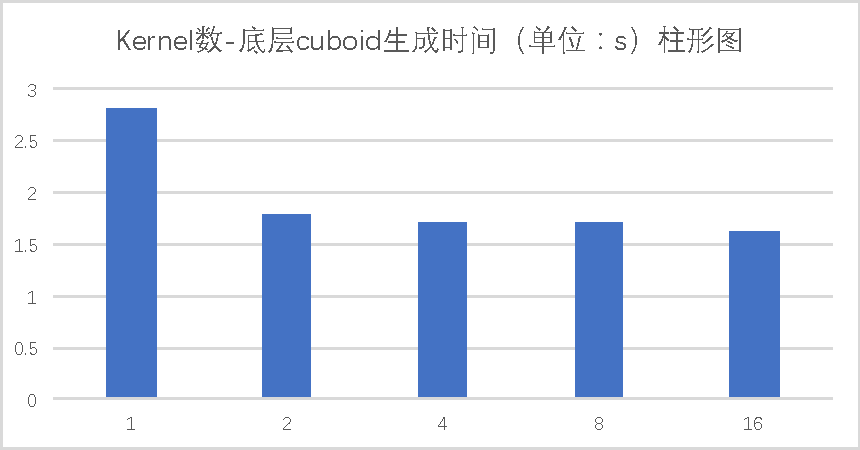
\includegraphics{CPU-KernelNumber-cuboidGenerate}
\caption{CPU:Kernel数-底层cuboid生成时间(单位:s)柱形图} 
\label{fig:figure1}
\end{figure}

另外,对于不同规模的数据集的测试有结果如下(基于kernel数=16)

\begin{table}[!htbp]
\centering
\caption{CPU:数据集大小-底层cuboid生成时间(单位:s)表} 
\label{tab:table5}
\begin{tabular}{|c|c|}
    \hline
    数据集条目数 & 计算部分的运行时间(s)\\
    \hline
    262144 & 0.0260788\\
    \hline
    2097152 & 0.06733256\\
    \hline
    16777216 & 0.3991288\\
    \hline
    134217728 & 1.62508\\
    \hline
\end{tabular}
% \note{这里是表的注释}
\end{table}

\begin{figure}[ht]
\centering
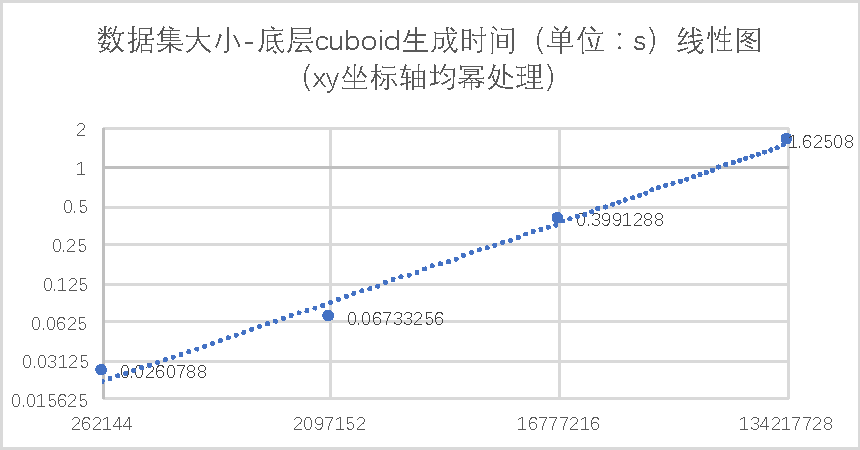
\includegraphics{CPU-DatasetSize-cuboidGenerate}
\caption{CPU:数据集大小-底层cuboid生成时间(单位:s)线性图} 
\label{fig:figure2}
\note{$x$, $y$轴均经过了幂处理}
\end{figure}

在不同的kernel运行时,从系统管理中能够查询到的内存空间占用如下表:

\begin{table}[htbp]
\centering
\caption{CPU:数据集大小-kernel数-内存占用(单位:MB)表} 
\label{tab:table6}
\begin{tabular}{|c|c|c|}
    \hline
    数据集条目数 & kernel数 & 总内存占用\\
    \hline
    262144 & 1 & 18.5\\
    \hline
    262144 & 2 & 25.0\\
    \hline
    262144 & 4 & 37.9\\
    \hline
    262144 & 8 & 63.8\\
    \hline
    262144 & 16 & 115.6\\
    \hline
    2097512 & 16 & 171.6\\
    \hline
    16777216 & 16 & 619.6\\
    \hline
\end{tabular}
% \note{这里是表的注释}
\end{table}

由上面这些测试数据和图表,可以得到如下结论:

1、由于该实验平台的CPU是$2$ core的,因此在多核实验中,生成的计算核心在超过$2$之后运行速度并没有实质性的变化(因为系统同时只能执行两个计算核心)。

2、另一方面,通过数据集大小和生成底层cuboid的时间的图表,可以看到这个算法运行的时间确实和原始数据集大小基本呈线性关系,与最初的算法分析一致。

在CPU-GPU架构上:

为了检验算法在更多核的平台上是否具有更好的可拓展性,因此该实验在GPU上重新部署了一遍。采用的数据集是$16777216$条目的数据集。具体的实验结果如下所示,其中所有的测量值都是五次测量的平均数。

\begin{table}[!htbp]
\centering
\caption{GPU:Kernel数-底层cuboid生成时间(单位:s)表} 
\label{tab:table7}
\begin{tabular}{|c|c|}
    \hline
    kernel数 & 计算部分的运行时间(s)\\
    \hline
    12 & 7.503698\\
    \hline
    16 & 6.260434\\
    \hline
    32 & 3.76185\\
    \hline
    48 & 2.971528\\
    \hline
    64 & 2.967586\\
    \hline
\end{tabular}
% \note{这里是表的注释}
\end{table}

\begin{figure}[ht]
\centering
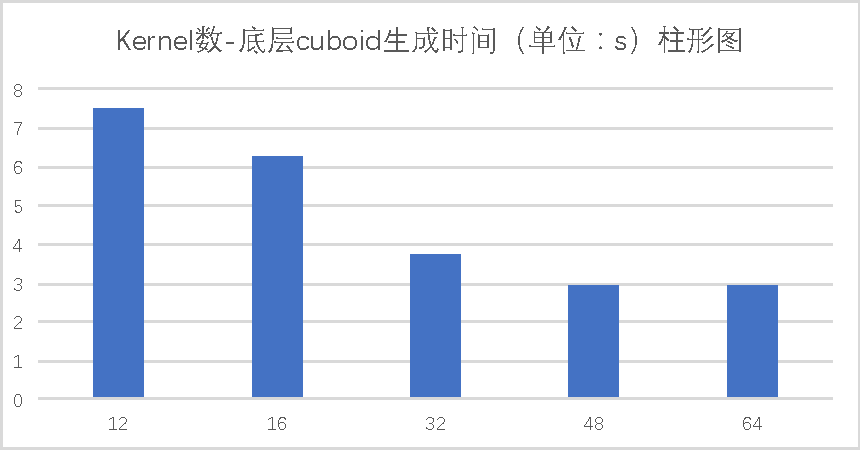
\includegraphics{GPU-KernelNumber-cuboidGenerate}
\caption{GPU:Kernel数-底层cuboid生成时间(单位:s)柱形图} 
\label{fig:figure3}
\end{figure}

由此可见,虽然实验结果的数值受限于硬件,仍然可以看出该并行算法具有很好的可拓展性,在具有更多(流)处理核心的并行计算平台上将获得更大的收益。

\subsection{对于由cuboid到cuboid的聚合算法的评估}

这一小节中将进行有无采用并行方式对于聚合性能的评估

在纯CPU架构上:

在本部分的测试中,我们将固定在cuboid聚合中使用聚合路线选择算法。采用的原始cuboid是基于$262144$个元素的数据集生成的cell总数为$24947$$(19, 101, 13)$的cuboid,目标cuboid是三步聚合后的顶层cuboid。另外,所有测试均采用下文将要测试的聚合路径优化算法。
测试结果如下:

\begin{table}[!htbp]
\centering
\caption{CPU:Kernel数-从cuboid到cuboid聚合时间(单位:s)表} 
\label{tab:table8}
\begin{tabular}{|c|c|}
    \hline
    kernel数 & 计算部分的运行时间(s)\\
    \hline
    1 & 0.001860436\\
    \hline
    2 & 0.001092724\\
    \hline
    4 & 0.00081602\\
    \hline
    8 & 0.000845582\\
    \hline
\end{tabular}
% \note{这里是表的注释}
\end{table}

\begin{figure}[ht]
\centering
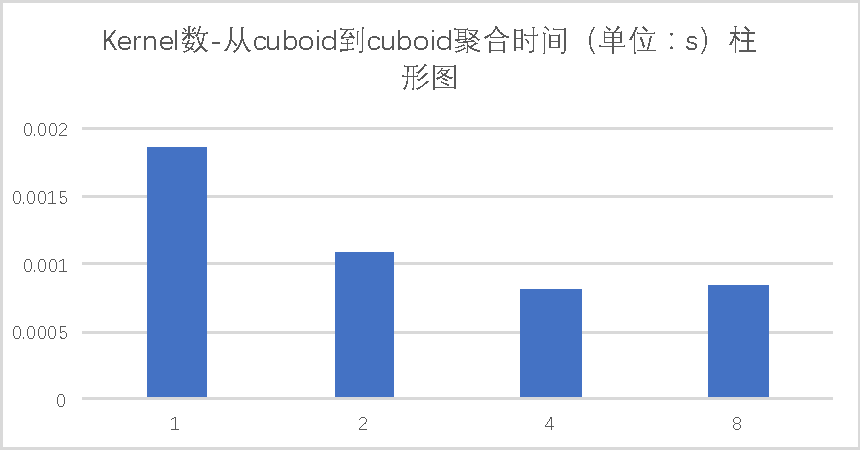
\includegraphics{CPU-KernelNumber-fromto}
\caption{CPU:Kernel数-从cuboid到cuboid聚合时间(单位:s)柱形图} 
\label{fig:figure4}
\end{figure}

在CPU-GPU架构上:
相同于之前的测试,这里我们仍然使用如下测试方法:原始cuboid是基于$262144$个元素的数据集生成的cell总数为$24947$$(19, 101, 13)$的cuboid,目标cuboid是三步聚合后的顶层cuboid。另外,所有测试均采用下文将要测试的聚合路径优化算法。
测试结果如下:

\begin{table}[!htbp]
\centering
\caption{GPU:Kernel数-从cuboid到cuboid聚合时间(单位:s)表} 
\label{tab:table9}
\begin{tabular}{|c|c|}
    \hline
    kernel数 & 计算部分的运行时间(s)\\
    \hline
    12 & 0.044490438\\
    \hline
    16 & 0.036521843\\
    \hline
    32 & 0.024351568\\
    \hline
    64 & 0.015527524\\
    \hline
\end{tabular}
% \note{这里是表的注释}
\end{table}

\begin{figure}[ht]
\centering
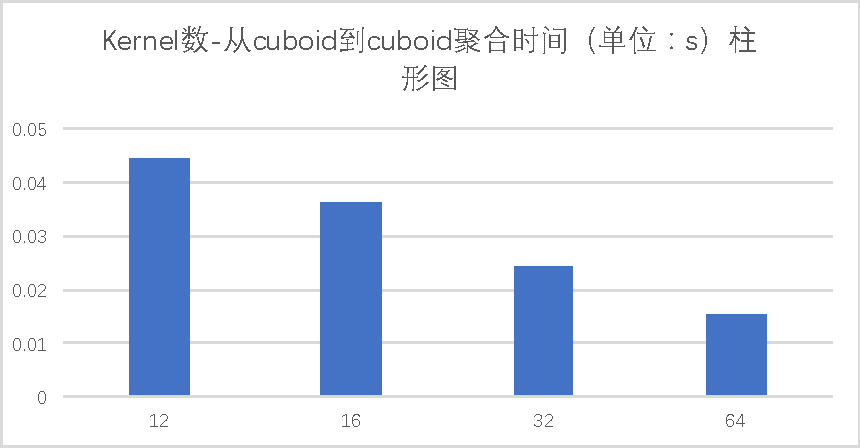
\includegraphics{GPU-KernelNumber-fromto}
\caption{GPU:Kernel数-从cuboid到cuboid聚合时间(单位:s)柱形图} 
\label{fig:figure5}
\end{figure}

从上述两组测量数据中也能够看出,并行之后的算法效率比起未并行之时有了很大的提升。另外,并行算法的良好的可扩展性也在实验数据中有所体现:其他条件相同的前提下,更高的并行数会带来更高的执行效率。

\subsection{对于聚合路线选择算法的评估}

在本小节中,我们将测试不同的聚合路线选择对于从一个较原始的cuboid到另一个上游cuboid的聚合性能的影响。

下文将列出参加测试的原始cuboid的各项参数,以及实际程序运行的结果。为了控制变量的原则,这里固定采用的硬件是CPU,OpenCL生成的计算kernel数为$16$。这些原始cuboid都是在之前的实中中生成的。为了简单起见,我们假定所有的聚合的最终目标都是一个“全维度聚合”cuboid,即一个顶层cuboid,从它将无法再进行任何聚合。

\begin{table}[!htbp]
\centering
\caption{CPU:聚合路径的选择与否系列图表(单位:s)表} 
\label{tab:table10}
\begin{tabular}{|c|c|c|c|c|c|}
    \hline
    原数据集条目数 & cell个数 & 路径优化 & 第一步 & 第二步 & 第三步\\
    \hline
    134217728 & 24947 & T & 0.00085184 & 0.00002840 & 0.00000615\\
    \hline
    134217728 & 24947 & F & 0.00082885 & 0.00010397 & 0.00001860\\
    \hline
    262144 & 24947 & T & 0.00085994 & 0.00002619 & 0.00000640\\
    \hline
    262144 & 24947 & F & 0.00083391 & 0.00016831 & 0.00001782\\
    \hline
    262144 & 3333 & T & 0.00027702 & 0.00000758 & 0.00000573\\
    \hline
    262144 & 3333 & F & 0.00026012 & 0.00004609 & 0.00002158\\
    \hline
\end{tabular}
% \note{这里是表的注释}
\end{table}

根据测试所得数据,可以做出柱形图来表现出各种不同的对比方式之间的性能差异。

\begin{figure}[ht]
\centering
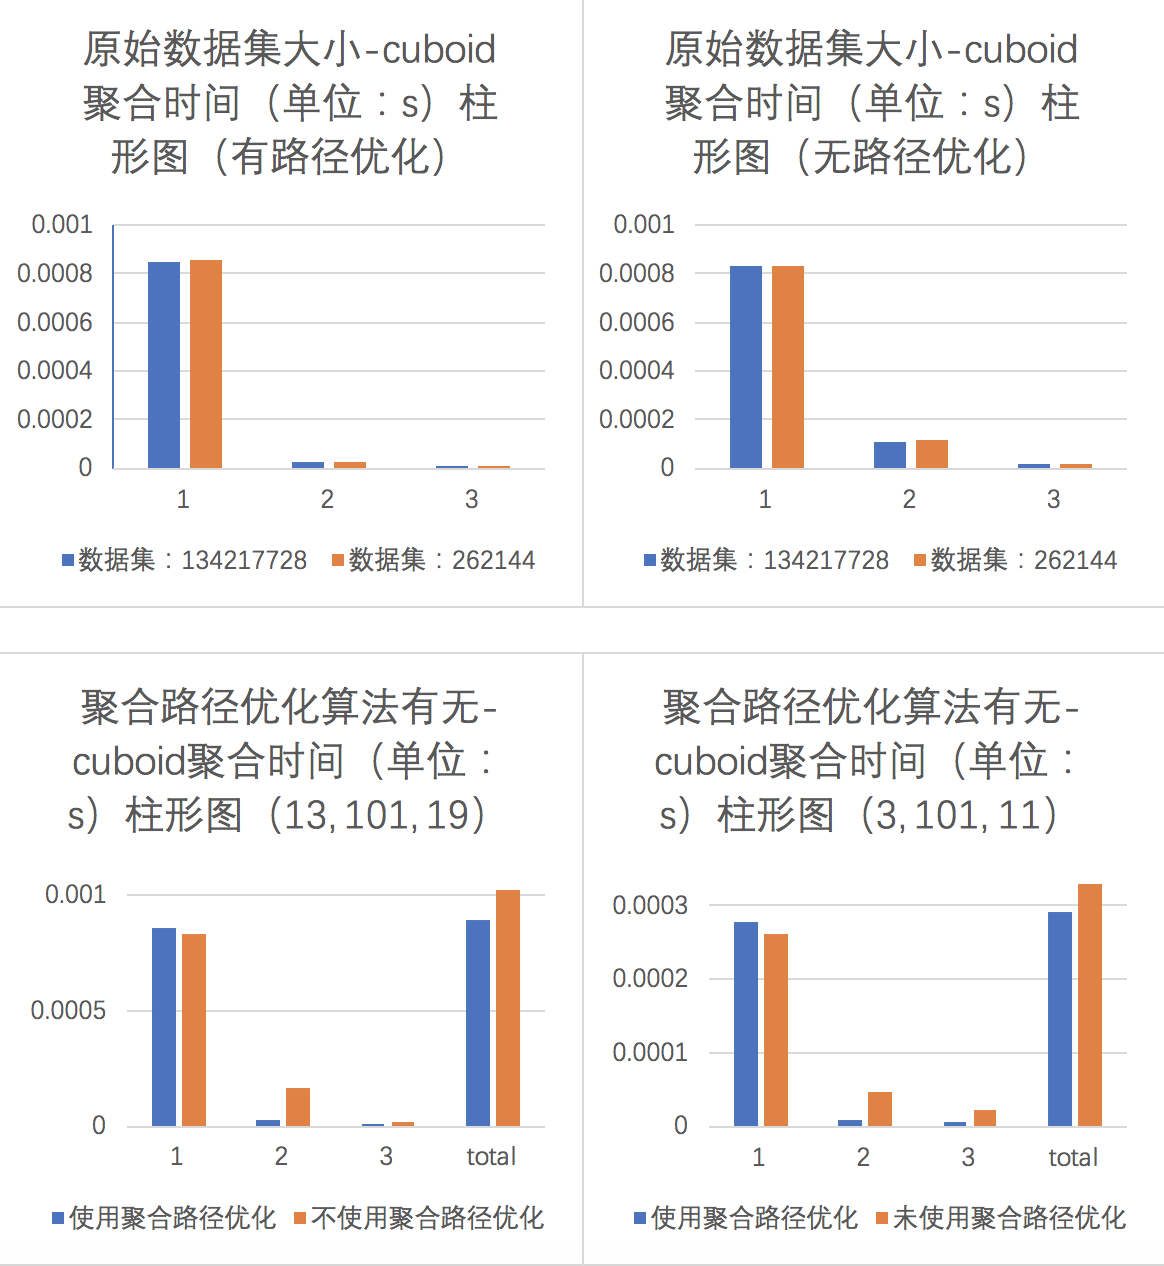
\includegraphics[width=10cm]{CPU-aggregateroute}
\caption{CPU:聚合路径的选择与否系列图表(单位:s)柱形图} 
\label{fig:figure6}
\end{figure}

可以从数据汇总表格和柱形图中看到如下规律:

1、由于这个算法是从cuboid出发的计算算法,因此与原始数据集的大小无关。

2、如同分析的那样,我们的路径优化算法在第一步聚合时是不会起到任何作用的,因此第一步的执行时间基本相同,可能由于系统架构或者是代码书写的问题,使用路径优化的方案甚至略慢于不使用路径优化的方案。而从第二步开始,经过了聚合路径优化的算法开始凌驾于未经过优化的算法。但是由于第一步聚合占用的时间占了整个聚合步骤的最主要部分,因此总体时间上来看优化的比例大概在10\%-15\%之间。

\subsection{花费函数在不同实验平台上的实际计算}

根据前文测试所得结果,下面我们分别在不同的平台上计算出一个花费函数,并且用这个花费函数与Stanford的方案下的花费函数来计算在不同情形下的预处理集合,以及评估他们之间的性能差距。

这个测试中,由于本身维度空间比较小(共$3$个维度),所以可能的cuboid总数$2^3 = 8$也并不是太多,因此在我们的测试中固定预处理的cuboid数量为$2$。评估最后的性能时,我们将以“除去底层cuboid以外的所有$7$个cuboid生成的总时间”作为评估标准。我们采用的底层cuboid的总cell数为$24947$,其中三个维度的值分别为$(19, 101, 13)$。另外,我们此处固定采用聚合路径优化算法。

在纯CPU架构上:

根据之前小节中估计的结果,我们已经有了花费函数估计式中的三个系数如下:

$C_{copy\_hd\_to\_m} = 9.34613 \times 10^{-8}$s / byte

$C_{init\_time} = 0.00225$s

$C_{copy\_d\_to\_m} = C_{copy\_m\_to\_d} = 4.70919 \times 10^{-10}$s / byte

考察$t_{scan\_per\_cell}$,其指的是在从cuboid到cuboid聚合时“单个kernel”对于“聚合前的单个cell”的处理时间。因此,这个地方要进行计算时,首先要选择的数据集应该也是“单kernel前提下”进行聚合的时间测量结果。因此我们将采用之前小节中聚合cuboid的测量数据进行计算。

测量表格中,给出的是“三步聚合的时间总和”,实际上我们在测量时也测量了第一步聚合的时间。我们在这里选择第一步聚合的时间作为我们的计算基准,是因为这样能尽可能平摊可能产生的系统与测量误差到每一个cell上,从而让我们的估计更为精确。

从实验数据中我们可以直接得到,在该平台上,对于$24947$个cell的扫描/聚合操作的总时间为$0.00184109$s,即$t_{scan\_per\_cell} = 0.00184109 \div 24947 = 7.38 \times 10^{-8}$s / cell

在CPU-GPU架构上:

根据之前小节中估计的结果,我们已经有了花费函数估计式中的三个系数如下:

$C_{copy\_hd\_to\_m} = 1.26069 \times 10^{-8}$s / byte

$C_{init\_time} = 0.195$s

$C_{copy\_d\_to\_m} = C_{copy\_m\_to\_d} = 1.7 \times 10^{-14}$s / byte

利用与之前类似的方法,也能计算出$t_{scan\_per\_cell} = 1.36165 \times 10^{-5}$s / cell

考察上一章中花费函数中提到的$count_A$与$count_B$,结合我们此处具体设置的实验条件,我们可以直接给出关于这两个量在所有情况下的具体取值。此时“cell的处理个数”指的是由原始cuboid到目标cuboid的路径上总共需要处理的cell个数。

\begin{table}[!htbp]
\centering
\caption{$count_A$表} 
\label{tab:table11}
\begin{tabular}{|l|l|}
    \hline
    目标cuboid的cell个数 & $count_A$(总共需处理的cell个数)\\
    \hline
    1919 & 24947\\
    \hline
    1313 & 24947\\
    \hline
    247 & 24947\\
    \hline
    101 & 24947 + 1313 = 26260\\
    \hline
    19 & 24947 + 247 = 25194\\
    \hline
    13 & 24947 + 247 = 25194\\
    \hline
    1 & 24947 + 247 + 13 = 25207\\
    \hline
\end{tabular}
% \note{这里是表的注释}
\end{table}

\begin{table}[!htbp]
\centering
\caption{$count_B$表} 
\label{tab:table12}
\begin{tabular}{|l|l|}
    \hline
    目标cuboid的cell个数 & $count_B$(总共需处理的cell个数)\\
    \hline
    1919 & 1919\\
    \hline
    1313 & 1313\\
    \hline
    247 & 247\\
    \hline
    101 & 1313 + 101 = 1414\\
    \hline
    19 & 247 + 19 = 266\\
    \hline
    13 & 247 + 13 = 260\\
    \hline
    1 & 247 + 13 + 1 = 261\\
    \hline
\end{tabular}
% \note{这里是表的注释}
\end{table}

于是,根据以上这些数据,我们可以计算出在两个不同的平台上的所有cuboid的$C(v)$了。

首先针对通常的database system,这样的system将预处理的cuboid缓存在硬盘等外部存储设备中。下面两个表格给出了我们计算出的$C(v)$值。第一列如同前述两个count的表格,均指的目标cuboid中的cell个数;第二列则直接列出根据前述花费函数公式,以及本小节中给出的常数值来计算的每个cuboid的花费值。

在纯CPU平台上:

\begin{table}[!htbp]
\centering
\caption{CPU + HD平台上的cell个数-$C(v)$表} 
\label{tab:table13}
\begin{tabular}{|l|l|}
    \hline
    将预处理cuboid的cell个数 & $C(v)$\\
    \hline
    1919 & -0.234726\\
    \hline
    1313 & -0.240735\\
    \hline
    247 & -0.251306\\
    \hline
    101 & -0.252971\\
    \hline
    19 & -0.253608\\
    \hline
    13 & -0.253666\\
    \hline
    1 & -0.253789\\
    \hline
\end{tabular}
% \note{这里是表的注释}
\end{table}

在CPU-GPU平台上:

\begin{table}[!htbp]
\centering
\caption{GPU + HD平台上的cell个数-$C(v)$表} 
\label{tab:table14}
\begin{tabular}{|l|l|}
    \hline
    将预处理cuboid的cell个数 & $C(v)$\\
    \hline
    1919 & -0.247233\\
    \hline
    1313 & -0.248049\\
    \hline
    247 & -0.249484\\
    \hline
    101 & -0.250798\\
    \hline
    19 & -0.250001\\
    \hline
    13 & -0.250009\\
    \hline
    1 & -0.250036\\
    \hline
\end{tabular}
% \note{这里是表的注释}
\end{table}

可以看出来,在我们的估计方案的基础上估计出来的$C(v)$和传统Stanford方案估计出来的不一样:并非按照cell个数而单调递增。

然后,在计算出来的$C(v)$值的基础上,我们会发现,实际上我们得到的$S$集合是一样的。这证明了我们的方案至少不会比Stanford原有的方案更差。具体关于这部分的原因会在接下来的小节中提到。

我们使用预处理的方案与未预处理的方案进行比对,能得到如下结果(运行在CPU平台上):

\begin{table}[!htbp]
\centering
\caption{CPU:预处理-全cuboid生成时间(单位:s)表} 
\label{tab:table15}
\begin{tabular}{|c|c|c|}
    \hline
    处理方式 & 预处理 & 未预处理\\
    \hline
    时间总和(读取文件+处理) & 0.289799 & 0.901132\\
    \hline
\end{tabular}
% \note{这里是表的注释}
\end{table}

\begin{figure}[ht]
\centering
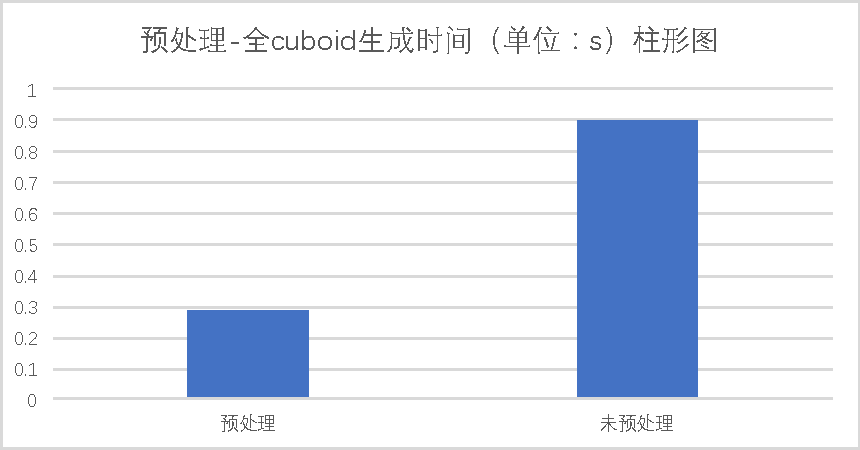
\includegraphics{CPU-preprocessing}
\caption{CPU:预处理-全cuboid生成时间(单位:s)柱形图} 
\label{fig:figure7}
\end{figure}

可以看到,进行了两次预处理之后,最占用运行时间的次低层cuboid的生成都被免去了,从而使得运行效率大幅度提高了。

接下来针对in-memory database模型,这样的database system会将尽可能多的有用信息缓存在memory中,从而使得对这部分数据的读写效率大幅提升。

首先计算这个前提下的$C(v)$。由于假定预处理完毕的cuboid现在存放在内存中,因此我们采用4.4.2.后半段提出来的适用于该情形的花费函数。该花费函数中没有$C_{copy\_hd\_to\_m}$一项。

以下是在该前提下计算出来的新的$C(v)$

在纯CPU平台上:

\begin{table}[!htbp]
\centering
\caption{CPU + in-memory平台上的cell个数-$C(v)$表} 
\label{tab:table16}
\begin{tabular}{|l|l|}
    \hline
    将预处理cuboid的cell个数 & $C(v)$\\
    \hline
    1919 & -0.00489118\\
    \hline
    1313 & -0.00485236\\
    \hline
    247 & -0.00478409\\
    \hline
    101 & -0.00499137\\
    \hline
    19 & -0.00481024\\
    \hline
    13 & -0.00480986\\
    \hline
    1 & -0.00481124\\
    \hline
\end{tabular}
% \note{这里是表的注释}
\end{table}

在CPU-GPU平台上:

\begin{table}[!htbp]
\centering
\caption{GPU + in-memory平台上的cell个数-$C(v)$表} 
\label{tab:table17}
\begin{tabular}{|l|l|}
    \hline
    将预处理cuboid的cell个数 & $C(v)$\\
    \hline
    1919 & -0.2162307387\\
    \hline
    1313 & -0.2162307373\\
    \hline
    247 & -0.2162307348\\
    \hline
    101 & -0.2173481446\\
    \hline
    19 & -0.21644094018\\
    \hline
    13 & -0.21644094016\\
    \hline
    1 & -0.2164520036\\
    \hline
\end{tabular}
% \note{这里是表的注释}
\end{table}

此时我们可以发现,$C(v)$的生成方式已经和Stanford有了很大的区别。在这个基础上计算出来的$S$集合如下:

Stanford:${24947, 247, 1313}$

我们的方案\_纯CPU:${24947, 1919, 1313}$

我们的方案\_CPU-GPU:(同上)

这里也能看出来,在CPU-GPU平台上,去掉了$C_{copy\_hd\_to\_m}$项之后,由于$C_{copy\_m\_to\_d}$项对$t_{scan\_per\_cell}$项影响实在微乎其微,因此整个式子的相对大小关系基本全部由扫描一项决定,即扫描的cuboid数($count_A$表)成为了$C(v)$差异的关键。而事实上由$count_A$表中也能看出来,由于聚合路径选择算法,使得后续步数的聚合远比前面一步的扫描要耗时更少,因此扫描的cuboid数量几乎没有差距,所以最终体现出来估计值几乎完全相同的情况。

最后,我们使用算法给出的预处理集合,分别测试两种预处理方案的性能差距。结果如下(运行在CPU平台上):

\begin{table}[!htbp]
\centering
\caption{CPU:预处理方式-全cuboid生成时间(单位:s)表} 
\label{tab:table18}
\begin{tabular}{|c|c|c|}
    \hline
    处理方式 & 我们的方式 & Stanford\\
    \hline
    时间总和(仅处理) & 0.00081504 & 0.00087807\\
    \hline
\end{tabular}
\note{在我们对in-memory模型的假定中,不存在硬盘读写}
\end{table}

\begin{figure}[ht]
\centering
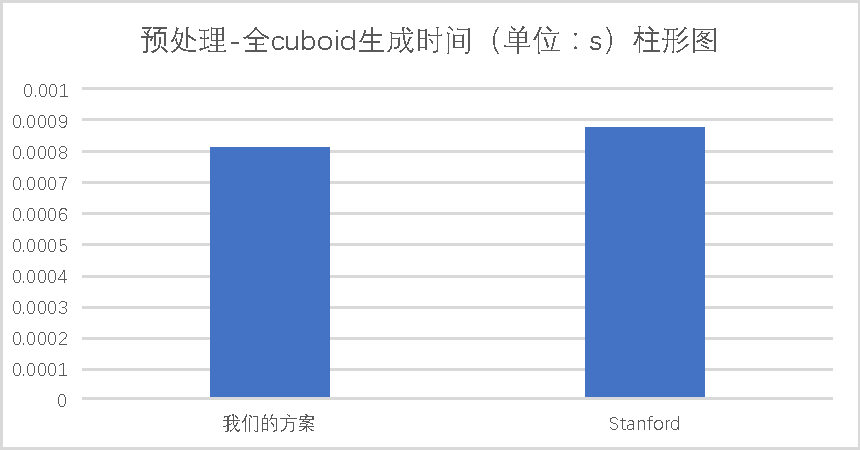
\includegraphics{CPU-preprocessing-approach}
\caption{CPU:预处理方式-全cuboid生成时间(单位:s)柱形图} 
\label{fig:figure8}
\end{figure}

可以看到,虽然差距不很明显,但是在这个场景设置下我们的预处理方案略优于Stanford提出的方案。

\section{实验分析与讨论}

\subsection{何时使用生成并行化的数据立方体生成的混合方案的考量}
在本小节中,我们将考察何时必须采用混合方案。

显然,若是条件允许,速度最优方案易于内存管理,易于程序流程控制并且拥有最高的运行速度,应该是我们的首选。而也如前所述,速度最优方案中的最大的问题在于潜在的占用内存空间过多问题。因此考察混合方案何时必须被使用,其实另一方面来说也是考察速度最优方案使用的边界条件。

在讨论内存空间问题的大前提下,我们可以发现,在整个算法运行之中,占用内存最多的主要是两块数据:直接读入的原始数据集,以及在运行中产生的临时subcuboid。下面就从这两个方面来分析其对于方案选择的影响。

在前面的的实验数据中,可以计算得出,在本实验所给定的cell的结构基础上,一个拥有$24947$个cell的cuboid所占用的空间约为$6.5$MB。因此仅从设备空间因素考虑,假定我们有$2$GB内存空间能够分配给这些临时subcuboid的前提下,能够同时运行的最大kernel数和一个cuboid的总cell数的关系大概如下:

\begin{table}[!htbp]
\centering
\caption{cell数目-最大可同时生成kernel数表} 
\label{tab:table19}
\begin{tabular}{|c|c|c|}
    \hline
    cuboid的cell的个数 & 最大可同时生成kernel数 & CPU or GPU\\
    \hline
    1000 & 7692 & GPU\\
    \hline
    5000 & 1538 & GPU\\
    \hline
    10000 & 769 & GPU\\
    \hline
    25000 & 307 & GPU\\
    \hline
    50000 & 153 & GPU\\
    \hline
    100000 & 76 & maybe GPU\\
    \hline
    250000 & 30 & maybe very good CPU\\
    \hline
    1000000 & 15 & CPU\\
    \hline
    2500000 & 6 & CPU\\
    \hline
    5000000 & 3 & CPU\\
    \hline
    7500000 & 1 & x\\
    \hline
\end{tabular}
\note{在我们对in-memory模型的假定中,不存在硬盘读写}
\end{table}

基本可以得到如下结论:在维度总乘积小于$100000$的时候,基本上可以不做任何调整将其部署在GPU上进行并行计算,正如本论文中实验所涉及到的数据集那样。在$100000$~$2500000$的区间,如果为了保证在GPU上的并行度,则应该转而采取混合方案来进行计算;而在CPU上仍可以采用直接计算的方法而不影响到并行度。在更大的区间上,则由于存储空间已经不足以支持数个,甚至是一个完整的cuboid,则无论CPU抑或是GPU都应该采取混合方案来进行计算。

然后,我们再来考察一下数据集大小对于是否采用混合方案的影响。然而实际上,由于本来就存在“原始数据集过大以至于无法一次全部读取”的问题,所以在内存的分配上,我们可以主要以cuboid占用的总空间作为衡量标准,然后对原dataset进行一定程度的划分,使得每个part的内存占用与临时subcuboid占用的空间总和不超过允许的最大限度。在此基础上,每次都在其中的一个part上运行我们的算法(然后我们的算法在运行过程中把这个part再分成一些更小的part),并将这个part的聚合结果暂时存储在一些其他存储介质中,最后再收集起来形成一个完整的数据集的底层cuboid。

综合以上两部分的分析,我们可以得知,采取何种方案其实直接相关于问题的规模,即我们需要得到的cuboid具体的cell总数的多少。然后在这个基础上,我们可以适当的在编程上对一次读入的数据集的大小进行调整,使得程序能尽可能更快地运行。

\subsection{对于修正后的花费函数的评估}

在本小节中,我们主要评估在不同的实验平台,也就是在不同的系数修正下得到的我们的估计花费函数和Stanford方案的差异点。

可以发现,实际上在硬盘性能不足,抑或是并行执行的算法计算量本身并非太大的话,对应项的系数修正之后,我们的方案的花费函数的最终表达式基本上和Stanford的式子是统一的:修正系数能让我们的花费函数的读写时间项的影响和别的项有超过1个数量级的差距,甚至更大。

而当我们在更宽的主板数据总线/更快的硬盘,或者直接忽略从外部存储到主存的时间(in-memory mode),抑或是运行更复杂的,计算量更大的并行算法的时候,系数的修正有时就会使得修正后的花费函数开始偏向于花费函数中的计算项或者是设备之间的拷贝项。此时两种花费函数所选择出来的预处理cuboid将有可能有所区别。而因为我们的花费函数直接以时间作为考量因素,因此在以时间作为衡量标准的最终运行效率上比以空间作为运行效率的间接考量因素的Stanford方案不会更差。

但无论怎样,我们的方案指出了一个事实:在不同的硬件平台,不同的算法构成的前提下,花费函数都是需要重新计算的。


\chapter{结论}
\citestyle{ustcnumerical}
本文提供了基于OpenCL的利用并行计算平台来对OLAP中数据聚合立方体的生成/计算进行优化的基本动机,设计方案,具体实现和评估结果。事实证明,采用了并行计算的方案在各方面都强于非并行方案,并且基于并行计算平台的特点而进行的一些优化也体现出了一定的效果。

未来该项研究的扩展方向将会往数个方向进行:重新审视花费函数,更加紧密结合并行计算平台的特点,提出更为通用的模型;将其扩展到CPU-GPU结合,或者是其他并行计算硬件的组合的异构计算平台;以及将以上这些技术整合成为一个更为完整的数据库系统。

\bibliography{bib/tex}

% \appendix
% \chapter{论文规范}

\backmatter
% \chapter{图片}
本章展示图片相关用法。

\section{示例}
\begin{figure}[ht]
\centering

\includegraphics[width=10cm]{ustc_logo_fig}
\caption{测试图片} \label{fig:figure1}
\end{figure}

\section{带图注的图}
\begin{figure}[ht]
\centering

\includegraphics[width=10cm]{ustc_logo_fig}
\caption{带图注的图片}\label{fig:noted-figure}
\note{the solid lines represent the time histogram of the spontaneous activities of an old monkey cell(gray) and a young monkey cell (black). The bin-width is 1}
\end{figure}

% \chapter{表格}

\section{A Simple Table}
\begin{table}[htbp]
\centering
\caption{这里是表的标题} \label{tab:simpletable}
\begin{tabular}{|c|c|}
    \hline
    a & b \\
    \hline
    c & d \\
    \hline
\end{tabular}
\note{这里是表的注释}
\end{table}

\section{长表格}
\begin{longtable}{ccc}
% 首页表头
\caption[长表格演示]{长表格演示} \label{tab:longtable} \\
\toprule[1.5pt]
名称  & 说明 & 备注\\
\midrule[1pt]
\endfirsthead
% 续页表头
\caption[]{长表格演示(续)} \\
\toprule[1.5pt]
名称  & 说明 & 备注 \\
\midrule[1pt]
\endhead
% 首页表尾
\hline
\multicolumn{3}{r}{\small 续下页}
\endfoot
% 续页表尾
\bottomrule[1.5pt]
\endlastfoot

AAAAAAAAAAAA   &   BBBBBBBBBBB   &   CCCCCCCCCCCCCC   \\
AAAAAAAAAAAA   &   BBBBBBBBBBB   &   CCCCCCCCCCCCCC   \\
AAAAAAAAAAAA   &   BBBBBBBBBBB   &   CCCCCCCCCCCCCC   \\
AAAAAAAAAAAA   &   BBBBBBBBBBB   &   CCCCCCCCCCCCCC   \\
AAAAAAAAAAAA   &   BBBBBBBBBBB   &   CCCCCCCCCCCCCC   \\
AAAAAAAAAAAA   &   BBBBBBBBBBB   &   CCCCCCCCCCCCCC   \\
AAAAAAAAAAAA   &   BBBBBBBBBBB   &   CCCCCCCCCCCCCC   \\
AAAAAAAAAAAA   &   BBBBBBBBBBB   &   CCCCCCCCCCCCCC   \\
AAAAAAAAAAAA   &   BBBBBBBBBBB   &   CCCCCCCCCCCCCC   \\
AAAAAAAAAAAA   &   BBBBBBBBBBB   &   CCCCCCCCCCCCCC   \\
AAAAAAAAAAAA   &   BBBBBBBBBBB   &   CCCCCCCCCCCCCC   \\
AAAAAAAAAAAA   &   BBBBBBBBBBB   &   CCCCCCCCCCCCCC   \\
AAAAAAAAAAAA   &   BBBBBBBBBBB   &   CCCCCCCCCCCCCC   \\
AAAAAAAAAAAA   &   BBBBBBBBBBB   &   CCCCCCCCCCCCCC   \\
AAAAAAAAAAAA   &   BBBBBBBBBBB   &   CCCCCCCCCCCCCC   \\
AAAAAAAAAAAA   &   BBBBBBBBBBB   &   CCCCCCCCCCCCCC   \\
AAAAAAAAAAAA   &   BBBBBBBBBBB   &   CCCCCCCCCCCCCC   \\
AAAAAAAAAAAA   &   BBBBBBBBBBB   &   CCCCCCCCCCCCCC   \\
AAAAAAAAAAAA   &   BBBBBBBBBBB   &   CCCCCCCCCCCCCC   \\
AAAAAAAAAAAA   &   BBBBBBBBBBB   &   CCCCCCCCCCCCCC   \\
AAAAAAAAAAAA   &   BBBBBBBBBBB   &   CCCCCCCCCCCCCC   \\
AAAAAAAAAAAA   &   BBBBBBBBBBB   &   CCCCCCCCCCCCCC   \\
AAAAAAAAAAAA   &   BBBBBBBBBBB   &   CCCCCCCCCCCCCC   \\
AAAAAAAAAAAA   &   BBBBBBBBBBB   &   CCCCCCCCCCCCCC   \\
AAAAAAAAAAAA   &   BBBBBBBBBBB   &   CCCCCCCCCCCCCC   \\
AAAAAAAAAAAA   &   BBBBBBBBBBB   &   CCCCCCCCCCCCCC   \\
AAAAAAAAAAAA   &   BBBBBBBBBBB   &   CCCCCCCCCCCCCC   \\
AAAAAAAAAAAA   &   BBBBBBBBBBB   &   CCCCCCCCCCCCCC   \\
AAAAAAAAAAAA   &   BBBBBBBBBBB   &   CCCCCCCCCCCCCC   \\
AAAAAAAAAAAA   &   BBBBBBBBBBB   &   CCCCCCCCCCCCCC   \\
AAAAAAAAAAAA   &   BBBBBBBBBBB   &   CCCCCCCCCCCCCC   \\
AAAAAAAAAAAA   &   BBBBBBBBBBB   &   CCCCCCCCCCCCCC   \\
AAAAAAAAAAAA   &   BBBBBBBBBBB   &   CCCCCCCCCCCCCC   \\
AAAAAAAAAAAA   &   BBBBBBBBBBB   &   CCCCCCCCCCCCCC   \\
AAAAAAAAAAAA   &   BBBBBBBBBBB   &   CCCCCCCCCCCCCC   \\
AAAAAAAAAAAA   &   BBBBBBBBBBB   &   CCCCCCCCCCCCCC   \\
\end{longtable}

% \chapter{数学}

\section{定理、引理和证明}

\begin{definition}
    If the integral of function $f$ is measurable and non-negative, we define
    its (extended) \textbf{Lebesgue integral} by
    \begin{equation}
        \int f = \sup_g \int g,
    \end{equation}
    where the supremum is taken over all measurable functions $g$ such that
    $0 \leq g \leq f$, and where $g$ is bounded and supported on a set of
    finite measure.
\end{definition}

\begin{example}
    Simple examples of functions on $\mathbb{R}^d$ that are integrable
    (or non-integrable) are given by
    \begin{equation}
        f_a(x) =
        \begin{cases}
            |x|^{-a} & \text{if } |x| \leq 1,\\
            0 & \text{if } x > 1.
        \end{cases}
    \end{equation}
    \begin{equation}
        F_a(x) = \frac{1}{1 + |x|^a}, \qquad \text{all } x \in \mathbb{R}^d.
    \end{equation}
    Then $f_a$ is integrable exactly when $a < d$, while $F_a$ is integrable
    exactly when $a > d$.
\end{example}

\begin{lemma}[Fatou]
    Suppose $\{f_n\}$ is a sequence of measurable functions with $f_n \geq 0$.
    If $\lim_{n \to \infty} f_n(x) = f(x)$ for a.e. $x$, then
    \begin{equation}
        \int f \leq \liminf_{n \to \infty} \int f_n.
    \end{equation}
\end{lemma}

\begin{remark}
    We do not exclude the cases $\int f = \infty$,
    or $\liminf_{n \to \infty} f_n = \infty$.
\end{remark}

\begin{corollary}
    Suppose $f$ is a non-negative measurable function, and $\{f_n\}$ a sequence
    of non-negative measurable functions with
    $f_n(x) \leq f(x)$ and $f_n(x) \to f(x)$ for almost every $x$. Then
    \begin{equation}
        \lim_{n \to \infty} \int f_n = \int f.
    \end{equation}
\end{corollary}

\begin{proposition}
    Suppose $f$ is integrable on $\mathbb{R}^d$. Then for every $\epsilon > 0$:
    \begin{enumerate}
        \renewcommand{\theenumi}{\roman{enumi}}
        \item There exists a set of finite measure $B$ (a ball, for example) such that
        \begin{equation}
            \int_{B^c} |f| < \epsilon.
        \end{equation}
        \item There is a $\delta > 0$ such that
        \begin{equation}
            \int_E |f| < \epsilon \qquad \text{whenever } m(E) < \delta.
        \end{equation}
    \end{enumerate}
\end{proposition}

\begin{theorem}
    Suppose $\{f_n\}$ is a sequence of measurable functions such that
    $f_n(x) \to f(x)$ a.e. $x$, as $n$ tends to infinity.
    If $|f_n(x)| \leq g(x)$, where $g$ is integrable, then
    \begin{equation}
        \int |f_n - f| \to 0 \qquad \text{as } n \to \infty,
    \end{equation}
    and consequently
    \begin{equation}
        \int f_n \to \int f \qquad \text{as } n \to \infty.
    \end{equation}
\end{theorem}

\begin{proof}
    Trivial.
\end{proof}



\section{自定义}

\newtheorem*{axiomofchoice}{Axiom of choice}
\begin{axiomofchoice}
    Suppose $E$ is a set and ${E_\alpha}$ is a collection of
    non-empty subsets of $E$. Then there is a function $\alpha
    \mapsto x_\alpha$ (a ``choice function'') such that
    \begin{equation}
        x_\alpha \in E_\alpha,\qquad \text{for all }\alpha.
    \end{equation}
\end{axiomofchoice}

\newtheorem{observation}{Observation}
\begin{observation}
    Suppose a partially ordered set $P$ has the property
    that every chain has an upper bound in $P$. Then the
    set $P$ contains at least one maximal element.
\end{observation}
\begin{proof}[A concise proof]
    Obvious.
\end{proof}

% \chapter{算法环境}
模板中使用 \texttt{algorithm2e} 宏包实现算法环境。关于该宏包的具体用法,
请阅读宏包的官方文档。

\begin{algorithm}[htbp]
\SetAlgoLined
\KwData{this text}
\KwResult{how to write algorithm with \LaTeX2e }

initialization\;
\While{not at end of this document}{
    read current\;
    \eIf{understand}{
        go to next section\;
        current section becomes this one\;
    }{
        go back to the beginning of current section\;
    }
}
\caption{算法示例1}
\label{algo:algorithm1}
\end{algorithm}

\IncMargin{1em}
\begin{algorithm}
\SetKwData{Left}{left}\SetKwData{This}{this}\SetKwData{Up}{up}
\SetKwFunction{Union}{Union}\SetKwFunction{FindCompress}{FindCompress}
\SetKwInOut{Input}{input}\SetKwInOut{Output}{output}

\Input{A bitmap $Im$ of size $w\times l$}
\Output{A partition of the bitmap}
\BlankLine
\emph{special treatment of the first line}\;
\For{$i\leftarrow 2$ \KwTo $l$}{
    \emph{special treatment of the first element of line $i$}\;
    \For{$j\leftarrow 2$ \KwTo $w$}{\label{forins}
        \Left$\leftarrow$ \FindCompress{$Im[i,j-1]$}\;
        \Up$\leftarrow$ \FindCompress{$Im[i-1,]$}\;
        \This$\leftarrow$ \FindCompress{$Im[i,j]$}\;
        \If(\tcp*[h]{O(\Left,\This)==1}){\Left compatible with \This}{\label{lt}
            \lIf{\Left $<$ \This}{\Union{\Left,\This}}
            \lElse{\Union{\This,\Left}}
        }
        \If(\tcp*[f]{O(\Up,\This)==1}){\Up compatible with \This}{\label{ut}
        \lIf{\Up $<$ \This}{\Union{\Up,\This}}
        \tcp{\This is put under \Up to keep tree as flat as possible}\label{cmt}
        \lElse{\Union{\This,\Up}}\tcp*[h]{\This linked to \Up}\label{lelse}
        }
    }
    \lForEach{element $e$ of the line $i$}{\FindCompress{p}}
}
\caption{算法示例2}\label{algo_disjdecomp}
\label{alog:algorithm2}
\end{algorithm}\DecMargin{1em}

% \chapter{代码环境}
模板中使用 \texttt{listings} 宏包实现代码环境。详细用法见宏包的官方说明文档。

以下是代码示例,可以在文中任意位置引用\autoref{code:first-code} 。
\begin{lstlisting}[language=C, caption=示例代码, label={code:first-code}]
#include <stdio.h>

int main( )
{
    printf("hello, world\n");
    return 0;
}
\end{lstlisting}

% \chapter{交叉引用}

图~\ref{fig:figure1} 位于第~\pageref{fig:figure1}~页,
其标题为\nameref{fig:figure1}。

表~\ref{tab:longtable} 位于第~\pageref{tab:longtable}~页,
其标题为\nameref{tab:longtable}。

代码~\ref{code:first-code} 位于第~\pageref{code:first-code}~页,
其标题为\nameref{code:first-code}。

算法~\ref{algo:algorithm1} 位于第~\pageref{algo:algorithm1}~页,
其标题为\nameref{algo:algorithm1}。

% \chapter{引用文献标注}

\section{著者-出版年制标注法}

\noindent
\verb|\citestyle{ustcauthoryear}|
\citestyle{ustcauthoryear}

\noindent
\begin{tabular}{l@{\quad$\Rightarrow$\quad}l}
  \verb|\cite{knuth86a}| & \cite{knuth86a}\\
  \verb|\citet{knuth86a}| & \citet{knuth86a}\\
  \verb|\citet[chap.~2]{knuth86a}| & \citet[chap.~2]{knuth86a}\\[0.5ex]
  \verb|\citep{knuth86a}| & \citep{knuth86a}\\
  \verb|\citep[chap.~2]{knuth86a}| & \citep[chap.~2]{knuth86a}\\
  \verb|\citep[see][]{knuth86a}| & \citep[see][]{knuth86a}\\
  \verb|\citep[see][chap.~2]{knuth86a}| & \citep[see][chap.~2]{knuth86a}\\[0.5ex]
  \verb|\citet*{knuth86a}| & \citet*{knuth86a}\\
  \verb|\citep*{knuth86a}| & \citep*{knuth86a}\\
\end{tabular}

\noindent
\begin{tabular}{l@{\quad$\Rightarrow$\quad}l}
  \verb|\citet{knuth86a,tlc2}| & \citet{knuth86a,tlc2}\\
  \verb|\citep{knuth86a,tlc2}| & \citep{knuth86a,tlc2}\\
  \verb|\cite{knuth86a,knuth84}| & \cite{knuth86a,knuth84}\\
  \verb|\citet{knuth86a,knuth84}| & \citet{knuth86a,knuth84}\\
  \verb|\citep{knuth86a,knuth84}| & \citep{knuth86a,knuth84}\\
\end{tabular}

\section{顺序编码制标注法}

\noindent
\verb|\citestyle{ustcnumerical}|
\citestyle{ustcnumerical}

\noindent
\begin{tabular}{l@{\quad$\Rightarrow$\quad}l}
  \verb|\cite{knuth86a}| & \cite{knuth86a}\\
  \verb|\citet{knuth86a}| & \citet{knuth86a}\\
  \verb|\citet[chap.~2]{knuth86a}| & \citet[chap.~2]{knuth86a}\\[0.5ex]
  \verb|\citep{knuth86a}| & \citep{knuth86a}\\
  \verb|\citep[chap.~2]{knuth86a}| & \citep[chap.~2]{knuth86a}\\
  \verb|\citep[see][]{knuth86a}| & \citep[see][]{knuth86a}\\
  \verb|\citep[see][chap.~2]{knuth86a}| & \citep[see][chap.~2]{knuth86a}\\[0.5ex]
  \verb|\citet*{knuth86a}| & \citet*{knuth86a}\\
  \verb|\citep*{knuth86a}| & \citep*{knuth86a}\\
\end{tabular}

\noindent
\begin{tabular}{l@{\quad$\Rightarrow$\quad}l}
  \verb|\citet{knuth86a,tlc2}| & \citet{knuth86a,tlc2}\\
  \verb|\citep{knuth86a,tlc2}| & \citep{knuth86a,tlc2}\\
  \verb|\cite{knuth86a,knuth84}| & \cite{knuth86a,knuth84}\\
  \verb|\citet{knuth86a,knuth84}| & \citet{knuth86a,knuth84}\\
  \verb|\citep{knuth86a,knuth84}| & \citep{knuth86a,knuth84}\\
  \verb|\cite{knuth86a,knuth84,tlc2}| & \cite{knuth86a,knuth84,tlc2}\\
\end{tabular}

\section{其他形式的标注}

\noindent
\begin{tabular}{l@{\quad$\Rightarrow$\quad}l}
  \verb|\citealt{tlc2}| & \citealt{tlc2}\\
  \verb|\citealt*{tlc2}| & \citealt*{tlc2}\\
  \verb|\citealp{tlc2}| & \citealp{tlc2}\\
  \verb|\citealp*{tlc2}| & \citealp*{tlc2}\\
  \verb|\citealp{tlc2,knuth86a}| & \citealp{tlc2,knuth86a}\\
  \verb|\citealp[pg.~32]{tlc2}| & \citealp[pg.~32]{tlc2}\\
  \verb|\citenum{tlc2}| & \citenum{tlc2}\\
  \verb|\citetext{priv.\ comm.}| & \citetext{priv.\ comm.}\\
\end{tabular}

\noindent
\begin{tabular}{l@{\quad$\Rightarrow$\quad}l}
  \verb|\citeauthor{tlc2}| & \citeauthor{tlc2}\\
  \verb|\citeauthor*{tlc2}| & \citeauthor*{tlc2}\\
  \verb|\citeyear{tlc2}| & \citeyear{tlc2}\\
  \verb|\citeyearpar{tlc2}| & \citeyearpar{tlc2}\\
\end{tabular}

% \begin{publications}

\section*{已发表论文}

\begin{enumerate}
\item A A A A A A A A A
\item A A A A A A A A A
\item A A A A A A A A A
\end{enumerate}

\section*{待发表论文}

\begin{enumerate}
\item A A A A A A A A A
\item A A A A A A A A A
\item A A A A A A A A A
\end{enumerate}

\section*{研究报告}
\begin{enumerate}
\item A A A A A A A A A
\item A A A A A A A A A
\item A A A A A A A A A
\end{enumerate}

\end{publications}


\end{document}
